%   *******************************************************************
%   * THIS IS THE MAIN FILE--RUNNING LATEX ON "AllegThesis.tex" WILL  *
%   * GENERATE THE ENTIRE THESIS (ASSUMING YOU HAVE NOT RENAMED IT).  *
%   * IF YOU ARE USING BIBTEX, RUNNING BIBTEX ON "AllegThesis" SHOULD *
%   * GENERATE YOUR BIBLIOGRAPHY. SPECIFIC DETAILS DEPEND ON WHAT     *
%   * ENVIRONMENT AND TOOLS YOU ARE USING (E.G., TEXMAKER OR COMMAND  *
%   * LINE TOOLS LIKE PDFLATEX OR LATEXMK).                           *
%   *******************************************************************
%
% AllegThesis.tex
% by A. Thall
% 13 Feb 2003
%
% Revised by R. Roos
% Nov 2013
%
% Revised and Added to GitHub Classroom by G. Kapfhammer
% November 2017
%
% Revised by OBC
% November 2018
%
% This document provides a sample Senior Thesis template for use
% by students in Allegheny's Computer Science and Applied Computing programs.
%
%   *******************************************************************
%   * LOOK FOR BLOCK COMMENTS SUCH AS THIS ONE FOR AN EXPLANATION OF  *
%   * THIS DOCUMENT AND HOW TO MODIFY IT FOR YOUR OWN THESIS!         *
%   *                                                                 *
%   * ANY LINE BEGINNING WITH A "%" IS A LATEX COMMENT AND IS IGNORED *
%   * BY THE LATEX PROCESSOR. YOU ARE ENCOURAGED TO COMMENT YOUR OWN  *
%   * LATEX CODE TO HELP YOU REMEMBER WHY YOU DID THINGS A CERTAIN WAY*
%   *******************************************************************
%
%   ********************************************************************
%   * THE FIRST SECTION OF THE MAIN LATEX FILE IS THE "PREAMBLE." IT   *
%   * INSTRUCTS LATEX TO IMPORT SPECIAL PACKAGES FOR THINGS LIKE       *
%   * INCLUDING FIGURES,  COLORED TEXT, ETC.            *
%   * DEPENDING ON YOUR NEEDS, YOU MAY FIND IT NECESSARY TO USE PACK-  *
%   * AGES THAT ARE NOT INCLUDED IN THIS TEMPLATE. SIMPLY IMITATE THE  *
%   * "\usepackage{...}" COMMANDS SHOWN BELOW.                         *
%   ********************************************************************

%   ********************************************************************
%   * BEGINNING OF PREAMBLE:                                           *
%   ********************************************************************

\NeedsTeXFormat{LaTeX2e}
\documentclass[12pt]{report}

%   ********************************************************************
%   * ALL BUT ONE OF THE FOLLOWING 5 LINES SHOULD BE COMMENTED OUT.    *
%   * (NOT ALL OF THESE OPTIONS HAVE BEEN TESTED IN THIS REVISION!)    *
%   ********************************************************************

%\usepackage[bottom,single]{gatorthesis} % for final department copy
\usepackage[debug,draft,single]{gatorthesis} % for student workcopy
%\usepackage[single]{gatorthesis} % for student
%\usepackage[debug,draft,nolists,nofront,single]{gatorthesis} % more options

\usepackage{comment}     % provides a way to "comment out" sections in blocks
\usepackage{amsmath}     % special symbols
\usepackage{amssymb}     % more special symbols
\usepackage{epsfig}      % needed for including figures
\usepackage{url}
\usepackage{listings}
\usepackage[figure]{algorithm2e}
\usepackage{graphicx}
\usepackage{float}

%   ********************************************************************
%   * OPTIONAL: IF YOU WANT FINE CONTROL OVER HOW LATEX HYPHENATES     *
%   * CERTAIN WORDS, YOU CAN PUT WORDS IN A "\hyphenation" COMMAND AS  *
%   * SHOWN IN THE FOLLOWING EXAMPLE. OTHERWISE, YOU MAY JUST IGNORE   *
%   * THE NEXT COMMAND.                                                *
%   ********************************************************************

% EXAMPLE: Don't hyphenate the words "itself" or "linear". Hyphenate
%          "representations" only at the places indicated by the "-":

\hyphenation{itself repre-sen-tations linear}

%   ********************************************************************
%   * THE FOLLOWING COMMAND HAS BEEN DISABLED--IGNORE.                 *
%   ********************************************************************
% The following provides a box to surround the thesis statement
%\newenvironment{Thesis}%
%{\begin{Sbox}\begin{minipage}{.95\linewidth}}%
%{\end{minipage}\end{Sbox}\begin{center}\fbox{\TheSbox}\end{center}}

%   ********************************************************************
%   ********************************************************************
%   ***  END OF PREAMBLE.                                            ***
%   ********************************************************************
%   ********************************************************************

%   ********************************************************************
%   * DOCUMENT CONTENT STARTS AT THE "\begin{document}" COMMAND:       *
%   ********************************************************************

\begin{document}

%   ********************************************************************
%   * FILL IN THE "{...}" BELOW WITH YOUR INFORMATION.                 *
%   ********************************************************************

\thesistitle{Automatic Detection of Pseudo-Tested Methods in a Test Suite Using Fault Injection}

\thesisauthor{Nicholas Tocci} \thesisadvisor{Dr. Gregory Kapfhammer}

\thesisnumber{CS2019-15} % SEE PAULINE LANZINE TO GET YOUR REPORT NUMBER!

\thesisreadera{Dr. Aravind Mohan}

%   ********************************************************************
%   * IN RARE CASES YOU MAY HAVE MORE THAN TWO READERS, IN WHICH CASE  *
%   * YOU SHOULD UN-COMMENT THE FOLLOWING AND ADD NAMES:               *
%   ********************************************************************
% \thesisreaderb{Dr. Your Third reader}
% \thesisreaderc{Dr. Your Fourth reader}

%   ********************************************************************
%   * YOU MAY IGNORE THE FOLLOWING COMMAND:                            *
%   ********************************************************************
\date{\FileRevised \\ $\mbox{}$Revision: 1.8 $\mbox{}$}

\thesismaketitle         % Creates the title page
\thesismakecopyright     % Creates the copyright page

%   ********************************************************************
%   * YOU MAY SPLIT YOUR THESIS INTO SEVERAL FILES AND "\include" THEM *
%   * AS SHOWN BELOW. FOR INSTANCE, FILE "abstract.tex" CONTAINS THE   *
%   * ABSTRACT, FILE "ack.tex" CONTAINS THE ACKNOWLEDGMENTS, ETC. YOU  *
%   * MAY, OF COURSE, PUT EVERYTHING INTO ONE HUGE FILE, BUT THERE ARE *
%   * ADVANTAGES TO SPLITTING THINGS UP--FOR EXAMPLE, YOU CAN COMMENT  *
%   * OUT "\include" LINES OF SOME PARTS IN ORDER TO PRINT DRAFTS      *
%   * CONTAINING SELECTED SECTIONS OF YOUR THESIS, SAVING PAPER AND    *
%   * PRINTING COSTS.                                                  *
%   *                                                                  *
%   * YOU ARE NOT REQUIRED TO HAVE A "dedication"--IF YOU DON'T, JUST  *
%   * DELETE THAT LINE OR COMMENT IT OUT WITH A LEADING "%"            *
%   ********************************************************************

\begin{abstract}
Large-scale systems are very complex and because of that, it is
very difficult to test them adequately. The current metric to determine if a system
has been thoroughly tested is called coverage. Test coverage as a metric can be a misleading
number that can cause test suites to be ineffective without the creator knowing.
Coverage is used to explain how much of a program is tested, but this does not
reveal whether or not the tests are adequate. This is an industry-wide issue as
many companies will not allow pull requests if the test coverage is any lower
than 100\%\cite{prause2017100}. This limitation can potentially lead to
something called a pseudo-tested method. A pseudo-tested method is a method that
is tested, but which passes regardless of the output of a function. So if a test passes without ensuring that the
output was as intended by the developer, that is a pseudo-tested method because it is believed that
the test is effective. A tool has been created, aptly named Function-Fiasco, that
helps determine how much of the code is adequately tested and provides a
metric that is more representative of the actual conditions of the system. The
tool is based on the idea of fault injection. Software fault injection denotes the artificial insertion, or injection, of faults and error states into a running software system~\cite{feinbube2018software}. The tool allows a function to run, but collects the output, and then
randomizes the output. It then runs the tests associated to the function using randomized output and if the test still passes, it is
a pseudo-tested method. It then produces a metric that is
representative of the behavior of the system. This study also has a completed analysis of this
information to determine if the system was accurate in detecting pseuodo-tested
methods.
\end{abstract}
  % REQUIRED!

% \include{dedication} % OPTIONAL

 \section*{Acknowledgments}
I would like to thank my friends and family for their support throughout this process. They were very helpful in keeping me enthusiastic about my research. I would also like to acknowledge the faculty of the Computer Science Department of Allegheny College, in particular, Dr. Gregory Kapfhammer. He was very influential and encouraging throughtout the implementation of the tool and the documentation of the research. Lastly, I would like to thank Allegheny College itself for providing me with an avenue for researching such an interesting topic.
       % OPTIONAL, BUT ALMOST EVERYONE INCLUDES IT

%   ********************************************************************
%   * FRONT MATTER--TABLE OF CONTENTS, ETC. YOU PROBABLY DON'T NEED TO *
%   * CHANGE ANY OF THIS UNLESS YOU HAVE NO TABLES OR FIGURES, OR YOU  *
%   * WANT TO CHANGE NUMBERING DEPTH FOR SUBSECTIONS, OR ...           *
%   ********************************************************************

\setcounter{tocdepth}{2}    % # of section levels shown in table of contents
\setcounter{secnumdepth}{3} % # of numbered subsection levels in the text

\tableofcontents
%\listoftables       % OMIT THIS IF YOU DON'T HAVE ANY TABLES
\listoffigures      % OMIT THIS IF YOU DON'T HAVE ANY FIGURES

%   ********************************************************************
%   * A GLOSSARY IS ALMOST NEVER NEEDED UNLESS YOU HAVE AN UNUSUALLY   *
%   * LARGE NUMBER OF SPECIAL TERMS OR NOTATIONS AND IT WOULD DETRACT  *
%   * TOO MUCH FROM THE FLOW OF THE PAPER TO DEFINE THEM IN-LINE.      *
%   ********************************************************************
%\include{glossary}  % OMIT THIS IF YOU DON'T HAVE A GLOSSARY (FEW PEOPLE DO)

%   ********************************************************************
%   * THE FOLLOWING "lstset" COMMAND IS ADAPTED FROM ONE FOUND AT:     *
%   * http://tex.stackexchange.com/questions/115467/                   *
%   * listings-highlight-java-annotations                              *
%   *                                                                  *
%   * SEE CHAPTER 3 AND APPENDIX A                                     *
%   ********************************************************************

\lstset{
  basicstyle=\footnotesize\tt, % the size of the fonts that are used for the code
  breakatwhitespace=false,     % automatic breaks only happen at whitespace?
  breaklines=true,             % sets automatic line breaking
  captionpos=b,                % sets the caption-position to bottom
  frame=single,                % adds a frame around the code
  language=Java,               % the language of the code
  keywordstyle=\bf,
  showspaces=false,
  showstringspaces=false,      % underline spaces within strings only?
  showtabs=false,
  tabsize=2                    % sets default tabsize to 2 spaces
}

%   ********************************************************************
%   * NOW INCLUDE THE CHAPTER FILES; COMMENT OUT ANY YOU DON'T WANT TO *
%   * PROCESS IN A PARTICULAR LATEX RUN.                               *
%   *                                                                  *
%   * INCLUDED FILES ARE ASSUMED TO END IN ".tex", E.G.,               *
%   * "ch01_overview.tex", "ch02_relatedwork.tex", ETC.                *
%   ********************************************************************

% ch:intro
%
% $Id: ch01_overview
%
%   *******************************************************************
%   * SEE THE MAIN FILE "AllegThesis.tex" FOR MORE INFORMATION.       *
%   *******************************************************************

\chapter{Introduction}\label{ch:intro} % we can refer to chapter by the label
Software systems are very complex in nature and because of this fact, they are very difficult to test. As Fred Brooks Jr. has said, ``Software entities are more complex for their size than perhaps any other human construct because no two parts are alike (at least above the statement level).''~\cite{brooks1987no} As a system grows, the interactions that each module has to the system becomes increasingly complex. Modules can become so interconnected that it may be hard to keep track of how different pieces of a system interact with each other let alone their functionality. Since many systems can be separated into modules and shared to other parts of the program, it is important to understand whether a system is working as intended by the  developer. To verify if the system has been implemented correctly, developers often look to testing.

% * What is Testing (DEF)
Software testing is a verification process for software quality assessment and software quality improvement~\cite{friedman_voas_1995}. The first way to check whether or not a system is functioning properly is to ask a simple question, ``Is it currently operating or has it crashed?'' Performing an eyeball examination of a system is a very helpful step in the process of verification. However, if the system is not crashed and there is no significant data incorrectness, it could be very easy to miss a system that is not operating properly. That is why eyeball examination, for the most part, has been replaced with Unit testing.

%   * What is Unit Testing
Unit testing is the process of testing different modules of the system in isolation~\cite{friedman_voas_1995}. This could entail taking one function, observing its inputs, and then testing it with an outcome that is understood and accepted. A simple example would be a function that takes in two numbers, \texttt{X} and \texttt{Y}, and multiplies them together. The test case would supply the numbers 2 and 3 to the function, and then assert that the result is 6. This example was written in the Python language with the Pytest framework and is illustrated in Listing \ref{testingExample}.

%       * Unit Testing Example
\begin{figure}[t!]
\begin{lstlisting}[language = Python, numbers = left, frame = single, caption = Example of a unit test in the Pytest~\cite{okken_2018} framework., label = testingExample]
calulator.py:
  def multiplication(x,y):
    product = x*y
    return product


test_calculator.py:
  def test_multiplication():
    x = 2
    y = 3
    multiplicationResult = multiplication(x,y)
    assert multiplicationResult == 6
\end{lstlisting}
\end{figure}

%   * Ensuring that the system is running the way that it is intended
The way that testing ensures that a system is running correctly is by passing or failing cases in a test suite, or a collection of test cases. A developer will write a test case that is meant to have a desired effect, and if the system produces something that is unexpected the test will fail. The developer can write multiple test cases that have different inputs to observe how the system behaves under differing conditions. Each test can have a different intended purpose, in the case of \ref{testingExample}, the developer can write a test case that provides a null variable or a zero to see if the system can detect those two issues and resolve them in the intended manner. The variations that a test can take changes depending upon the intended functionality of the method it is testing.

% * coverage
One of the most important questions is, ``How can I know that my test suite is of good quality?'' As of right now, the answer to that question is coverage.

%   * What is coverage
Code coverage is a measurement of what percentage of the code under scrutiny is being tested by a test suite~\cite{okken_2018}. This metric can be used to ensure that developers are writing enough test cases for their systems. It reveals how much of the system is not being observed by the test suite.

%   * How is coverage calculated
This metric can be calculated in a variety of different ways, each one of which serves its own purpose.
%     * Branch
Branch coverage is the  percent of all control sequences being completed during the testing of the system~\cite{zhu1997software}. Simply put, branch coverage is looking to observe if every path of decision trees is being executed during the test run. So if there is an if/else statement that is checking if a number is even or odd, the test suite needs to include a test case for each of these scenarios.

%     * Branch coverage calculation
        \begin{quote}
        \textbf{\textit{Definition:}} Branch coverage is the fraction of the total number of branches that have been executed by the test data~\cite{malaiya2002software}.

        \begin{equation}
        \mbox{\emph{Branch Coverage}} = \frac{\mbox{\emph{Tested Branches}}}{\mbox{\emph{Total Number of Branches}}}
        \end{equation}
        \end{quote}

%     * statement
Statement coverage is the most brute force code coverage metric. It is the  percent of statements that have been executed in the test suite. So if there are 100 statements in the system, and only 85 are being executed, the coverage check will reward the system with being 85 percent covered.

%     * Statement coverage calulation
\begin{quote}
\textbf{\textit{Definition:}} Statement Coverage is the fraction of the total number of statements that have been executed by the test data~\cite{malaiya2002software}.

\begin{equation}
\mbox{\emph{Statement Coverage}} = \frac{\mbox{\emph{Tested Statements}}}{\mbox{\emph{Total Number of Statements}}}
\end{equation}
\end{quote}
%     * function
One of the most useful types of coverage is the function coverage. This is the percentage of the functions in the system that have been executed in a test case. This is a very baseline example for the unit testing as mentioned before. Testing of each function helps developers know if the intended behavior within the functions that are helping the system run are performing as intended. The following equation is used to calculate this type of coverage:

%     * function coverage calculation
        \begin{quote}
        \textbf{\textit{Defintion:}} A method \textit{m} $\in$ \textit{P} is said to be covered if there exists at least
        one test case \textit{t} $\in$ \textit{TS}, the test suite of program \textit{P} that triggers the execution of at least one path of the
        body of \textit{m}. \textit{TS} is the test suite of \textit{P}~\cite{vera2017comprehensive}.

        Where (\textbf{\textit{TM}}) is the number of tested methods in \textit{P},

        \begin{equation}
        Function Coverage = \frac{TM}{NUMM}
        \end{equation}
        \end{quote}

%   * Why is coverage helpful
Checking the code coverage is a very important step in the development of a large scale system. It can help a developer understand what code needs to be tested, and ensures that there is at least one test case for every function. The need for a system with high coverage is important, but it does raise a very important question, ``Is there a way for a developer to know if they have a good test suite?''

%   * Why can coverage be misleading
Coverage is a very important measure, but it can be misleading. It is helpful to show a developer how much of their system has been covered by the test suite, but it does not provide any information on the test suite having high fault detection effectiveness. A test case that has a call to a function, but cannot detect a bug will still be counted as covered if the calculation was running under function coverage. ``Although 100\% branch coverage will make us feel better about the reliabilty than will 50 percent branch coverage, the true reliability of the code will be the same.~\cite{friedman_voas_1995}'' Parts of the system that are not being tested could include bugs that the developers have not yet found, or that the developer is not testing for. The subject that coverage leaves out of its calculations is pseudo-tested methods.

% * Pseudo-tested methods
%   * What is a pseudo-tested method and why is it an silent issue
A pseudo-tested method is a method that will still pass test cases when the effects of a method are suppressed~\cite{vera2017comprehensive}. Simply put, it is a test case that will never fail. A pseudo-tested method can heavily impact a system. If there is unexpected information given to a pseudo-tested method and it doesn't know how to handle it, either bad results will follow or the system could crash. The only indicator that a pseudo-tested method has been written is that a test will never fail, regardless of the inputs that it is taking. The issue with this indicator is that passing test cases is a good thing. Many developers will overlook a passing test case, simply because it is passing. This makes sense, it follows the idea of, ``if it isn't broken, don't fix it.'' Therein lies the problem with pseudo-tested methods. Why would a developer investigate something that does not indicate a problem in what they wrote? This is an interesting concept because the way that a pseudo-tested method can exist is by writing a test case that will never fail.

%   * They are really easy to write
It seems as though it would be difficult to write a test case for a method that will never fail, but it is actually very easy. Whether it comes from developer error or not testing for the right things, it is entirely possible to write this type of test case.
%   * What does a pseudo-tested method look like
A pseudo-tested method could be produced in a variety of different forms, but a version of human error is represented in Listing \ref{pseudo}. To explain the example, the method \texttt{numberCheck} is being pseudo-tested. The test is checking whether or not the function \texttt{numberOrder} is sorting a list of numbers that is given to it.  Unfortunately the test, whether or not intended, is testing the initial set of numbers when it should be testing the list of sorted numbers with what is returned. More importantly the test is using sets and not lists. In sets the order does not matter, in lists order is maintained. Therefore the test will never fail, even though a list of numbers that is not ordered is being compared to a list of numbers that is ordered. This example serves to show how simple it is to accidentally pseudo-test methods. This test is not analyzing the correct variable and is not using the correct datatype, but the test will never fail.

%   * Pseudo-tested method example
\begin{figure}[t!]
\begin{lstlisting}[language = Python, numbers = left, frame = single, caption = Example of a pseudo-tested method, label = pseudo]
numbers.py:
  def numberOrder(n):
    numbersSorted = sorted(n)
    return numbersSorted


test_numbers.py:
  def test_numbers_ordered():
    numbers = set([1,3,2,4])
    sortedNumbers = set([1,2,3,4])
    orderedNumbers = numberOrder(numbers)
    assert numbers == sortedNumbers
\end{lstlisting}
\end{figure}

Pseudo-testing as an action is the product of unknowingly creating a test that will always be satisfied. There are many reasons that this can occur, and this is a problem that exists in larger systems as well. Even large systems that maintain a very high coverage contain many pseudo-tested methods~\cite{vera2017comprehensive}. As stated before, this is because the metric that many of these larger systems rely on, coverage, could be a misleading metric. What are the circumstances for a pseudo-tested method to be created? One is a company that is expected to maintain a high level of code coverage. This could lead to employees writing a test case just to write a test case and fulfill the baseline requirements so that they may have their pull requests approved. This is an industry-wide issue as many companies will not allow pull requests if the test coverage is any lower than 100 \%\cite{prause2017100}. The other issue is having a test case pass and simply moving along without any further examination. If a developer does not know that they have written a pseudo-tested method, and has a passing test case, they may begin development somewhere else. Since this test would be considered covered, it would also be included in pull requests further affecting different portions of the system.

Since it is so easy to write a pseudo-tested method, what are the current ways for automatic detection of pseudo-tested methods? The short answer for the Python programming language is that there isn't one. There are really only two ways for determining the fault detection effectiveness in Python, and both are by hand. Observing that the inputs and outputs of the functions can become tedious by hand provides the possibility that there could be inputs that will still fail the test suite, but not be tested. The other way is to do a proof of correctness for the test suite. The main issue with this type of validation is that it can take a very long time, and by the time that there is a pseudo-tested method found, the functionality of that portion of the system could have changed. Even visually it is very hard to notice pseudo-tested methods if the developer is not specifically looking for them.

Since initially there was no way to detect pseudo-tested methods automatically or manually with any accuracy, this thesis introduces the Automatic Detection Tool: Function-Fiasco.

Function-Fiasco is a tool that analyzes Python programs that are tested with the Pytest framework~\cite{okken_2018} to automatically detect pseudo-tested methods. It will check every method that is in the program by supressing the behavior of the system to determine if the test is strong enough to detect when there are unexpected changes to the way the method works. Function-Fiasco uses a combination of fault-injection, fuzzing, and mutation testing to accurately assess a system's test suite to detect pseudo-tested methods. Function-Fiasco supports primitive data types to return a table that describes the coverage of the system as a percent of the amount that is covered, and represents the fault detection effectiveness.

Function-Fiasco was used on a group of 10 GitHub projects to determine its effectiveness and the amount of pseudo-tested methods that are present in Python based systems. The important contributions of this research are as follows:

\begin{enumerate}
  \item A working automatic detection tool for pseudo-tested methods for Python based systems.
  \item A table that contains the results of a system's coverage and fault detection effectiveness.
  \item A revised metric that describes how accurately a system is able to detect errors.
  \item Two Pytest plugins that aid in the testing of software.
\end{enumerate}

%
\section{Motivation} \label{sec:motivation}
%
% * Why testing is so important in general
Function-Fiasco was created because testing as a topic is very important. Testing is the way that developers will know how a certain condition will affect a system. A well tested system is stable and prepared for any unexpected changes to function inputs. This is the main reason that testing exists on every software engineering model. Without testing, developers would not know the true behaviors of the system and may have written a bug that could crash during execution or provide incorrect results to a user. While designing a system is a very important part of the development cycle, designing the test suite that it will be running beside and verifying its functionality could arguably be more important. Developers use test suites to ensure that the work that they are doing is correct and intended. This process can be broken into two different pieces. Validation is the process of ensuring that the sofware is doing the right thing and verification is the process of ensuring that the software is performing its purpose correctly~\cite{friedman_voas_1995}. In the past, much of the software assessment would be completed towards the end of the cycle. Function-Fiasco is still able to help systems that are being tested in this manner as it will help developers know if they are writing tests that will detect bugs. There has been a recent push towards a more \textit{test-first} mindset. Test-driven development is a rising idea in Software Development. In test-first development, the system is thought out and test cases are written prior to the writing of the software. Test-first development has many benefits, such as a greater organization and a better understanding of the flow of the system. Additionally, developers know when they have created software that fits the intended functionality of the system~\cite{fucci2017dissection}. Function-Fiasco is also able to help in Test-driven development. After a test has been written in the process of Test-driven development, functionality implementation begins. This is the process of understanding what a function needs to do and writing the implementation that will complete this process. Tests are often used to determine if a developer has written the right implementation. Function-Fiasco can be used at this stage. It can be used to determine if the tests will be able to detect all mutations that the code can take.

% * Has not been done in python before
The second most important reason for the creation of this tool is that nothing like it exists for the Python programming language. One other tool Descartes is a tool that automatically detects pseudo-tested methods in the Java programming language for systems~\cite{vera2018descartes}. This is the only other tool that analyzes systems for pseudo-tested methods, and since it is made for the Java programming language, it will not work on systems of other programming languages. Also, it has been explained that mutation testing results can be skewed by the programming language~\cite{vera2017comprehensive}. This can be explained by the different algorithms that different programming languages use and the idea of type safety. Programming languages, such as Java, that use strict typing will not overwrite a variable with a different type, like an \texttt{int} becoming a \texttt{char}. Python will perform such an operation, an example of this is in Listing 1.3, where the new value of \texttt{a} is the \texttt{String} instead of the \texttt{int}. The reasoning is Python does not require declarations to reserve memory space. Therefore there needs to be a tool that will detect pseudo-tested methods in Python.
% * needed metric for code testing

The next piece of motivation is the potential misleading nature of coverage. As mentioned before, as long as a function is called in a test suite, that function is considered covered. Coverage cannot give an indication of the fault detection effectiveness for a test suite, which is a very important part of testing. If there is no way to determine that a test suite is properly created, and developers have to rely solely on coverage as a validation metric, the easy creation of pseudo-tested methods will remain. One of the only ways to determine the fault detection effectiveness of a test suite is to do a check on each test case by hand and to run many different mutations for it. This type of work can be very time consuming and would create a unneccessarily long list of test cases that can become redundant. That is why many companies lean towards using coverage, as it implies that many mutations are covered in the test suite, when in reality it is only how much of the program is being executed in the test suite. Function-Fiasco generates a metric that is the overall coverage which is modified to reflect the number of pseudo-tested methods. This metric is representative of the overall behaviors in the system. It will allow developers to not only know how much of their system is covered, but it will also give them an idea to the fault detection effectiveness of their test suite.

\begin{figure}[t!]
\begin{lstlisting}[language = Python, numbers = left, frame = single, caption = Example of interpreted languages, label = interpreted]
inter.py:
  print("1")
  print("2")
  print("3")

\end{lstlisting}
\end{figure}

% * What is python?
The final reason that Function-Fiasco was created, is for the Python language. Python is quickly becomming one of the most popular languages in terms of job opportunities as shown in Figure \ref{languageGrowth}~\cite{wang2017computer}, which was generated using the Indeed Job Trends. Python is an interpreted, interactive, object-oriented programming language\cite{sanner1999python}. An interpreted language is a language that is compiled during runtime for errors, such as syntax. An example is Listing \ref{interpreted}. In this example, both the numbers 1 and 2 will print during the execution of the program. Then the system will encounter the incorrect syntax of the \texttt{print} statement and crash. Python is also a very loosely typed language, which means that variables can easily be overwritten. This loose type safety directs to the hypothesis of: \emph{Since Python is a loosely typed language, there could potentially be a higher concentration of pseudo-tested methods written into systems that are written in Python.} Another factor in in the choice for Python, was the Pytest framework. The reason that Python was the chosen language for Function-Fiasco is the growing popularity of the language.  Since it is becomming more popular and Python has loose type safety, there needs to be a tool that makes it easier for developers to know when they have written test cases that represent the fault detection effectiveness, and Function-Fiasco helps accomplish that. Function-Fiasco will indicate that test cases are still passing when they shouldn't. For example, if a developer is accidentally using the wrong datatype, as shown in Listing \ref{pseudo} and the test still passes, Function-Fiasco will be able to detect that.
\begin{figure}[htbp]
  \centering
  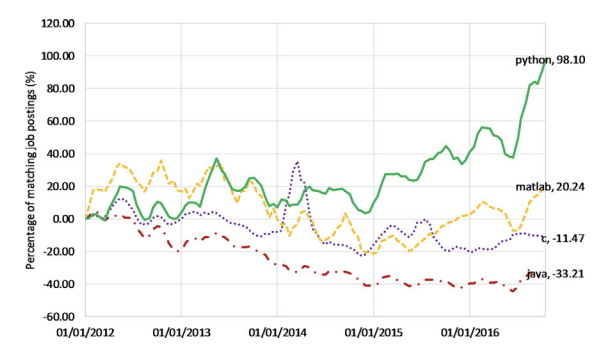
\includegraphics[width=5in]{images/language-growth.png}
  \caption{Job opportunities per language~\cite{wang2017computer}.}~\label{languageGrowth}
\end{figure}




%   * Explain the benefits of python
% * More valuable
% * why did I choose it


\section{Current State of the Art}\label{sec:stateofart}

As mentioned previously, the current state of the automatic detection for pseudo-tested methods is almost non-existant. Other than Function-Fiasco, there are three ways to detect a pseudo-tested method. Decartes is a tool that uses mutation testing to detect pseudo-tested methods, but this tool could only assist a developer if they are using Java. Descartes will not assist developers in any other programming language. Mutation testing is the process of changing code to produce a mutant that will be detected by the test case. If the mutant is not detected, a mutation score is calculated by using the ratio of detected mutants to total mutants. This score is representative of the test suite effectiveness. This score can be calculated as follows:

\begin{quote}
\begin{equation}
\mbox{\emph{Mutation Score}} = \frac{\mbox{\emph{Detected Mutants}}}{\mbox{\emph{Total Mutants}}}
\end{equation}
\end{quote}

It is important to note that the way that Function-Fiasco employs mutation testing is vastly different from Descartes. Decartes uses extreme mutations. Extreme mutation very simply removes all side effects of a function from the running of a system. In Decartes, if a function has a void return, all statements will be removed from the body of the function. If there is a return type, a pre-determined value is returned. This complete change is meant to be caught by the test suite. If it is not, the function is pseudo-tested~\cite{vera2018descartes}. Function-Fiasco does not affect the statements inside the body of a function at all. However, it does interact with functions, but only so that it may add decorators to indicate to Function-Fiasco where a mutation needs to occur. It will then allow the function to be run. This is so that it may determine the return type of the system, this is necessary as Python is a loosely-typed language. It will then randomize the value of the return so that the test suite is receiving an input that is not what was expected, but is of the correct type except in cases where a \texttt{boolean} is returned. So instead of a mutation of code structure or statements, there is a mutation of the inputs into the test suite.

The other way of detecting pseudo-tested methods is by checking each function by hand. A developer may look at a test suite to determine its inputs and expected output and run a visual test. This test will check if inputs that are known to produce a failing result will actually detect a failing result. If this result is passing, the function that is being tested is considered pseudo-tested. This process is very tedious and still has the impact of human error. Because a human is preparing the inputs that the test will receive, these tests may not be testing the right inputs, due to the potential for human error. For example, a test would pass if it receives a postive number, but the developer does not know that a negative number may pass as well. This developer can create five scenarios to test positive numbers, but never see that the test will pass even if it receives a negative number. The mutation for the inputs by a human always has an element for human error. One other significant issue with testing systems by hand is that the size and complexity of systems may make this work meaningless. Since this is a very time consuming task, depending on the size of the system, the functionality of the portion of the system that is being hand tested may change before the test determines if a function is being pseudo-tested.

The final way to detect for a pseudo-tested method is one that may sound dangerous, and it is: to not test for it at all. The idea of a pseudo-tested method is a relatively new topic. This is evident as the idea was introduced by Niedermayr and colleagues~\cite{niedermayr2016will}~\cite{vera2017comprehensive}. This means that there could be a plethora of systems in the field that have functions that are being pseudo-tested. This is a very frightening idea. Pseudo-tested methods are a relatively silent issue, which means that developers do not know about the dangers of them and are still writing them. Since many places are not testing for them at all, the way that the developers will realize that there is an issue with their test suite is when their system crashes or when certain results are not what was expected.

\section{Goals of the Project}\label{sec:goals}

% * there could be more pseudo-tested methods present in systems that are written using the python code base
%   * Prove that typed languages could contain less pseudo-tsted methods than typed languages
The first main goal of this research is to prove that there are pseudo-tested methods in systems that are written in loosely typed languages. The reasoning behind this goal is based around the syntax and semantics of strictly typed languages. For a loosely typed language, such as Python, variables can quickly be overwritten. So if a function is expecting a String, but it is given an integer, the system will not error, unless that variable is being used in a way that does not adhere to the data type. For a strictly typed language, this type of variable interaction will not be allowed. The system will produce an error, usually saying it was expecting a String, but received an int. Typed languages protect from interactions such as this, in a way forming a secondary test to ensure that the intended use of the function is followed. Loosely typed languages do not have this type of barrier, and may lead to the more concentrated creation of pseudo-tested methods.

% * explain the system that I have created to detect pseudo-tested methods in the pytest framework
This research was also meant to produce a tool that Python developers can use to ensure that the test suites they are creating have a high fault detection effectiveness. The tool can detect pseudo-tested methods automatically, which was not possible before. It was created in Python, for Python based systems that are being tested in the Pytest framework. Python was chosen because it is the fastest growing language and Pytest is one of the most popular testing frameworks, as indictated in Figure \ref{languageGrowth}. Function-Fiasco was meant to be used by the greatest number of people for the fastest growing systems, and is derived from multiple different testing techniques. These include: fault-injection, fuzzing, and mutation testing. This combination was intended to expose the systems that are being tested to the highest amount of observation so that pseudo-tested methods are detected. Afterwards, Function-Fiasco will deliver a table that is meant to serve as a report for the system.

% * create a metric that will allow developers in other languages to keep track of the fault detection effectiveness
The creation of a metric will allow developers to keep track of the fault detection effectiveness. One of the most significant issues in the field was that developers had to rely almost solely on coverage to determine if their test suite was of high quality. While it may have been in high quality for the amount of the system that was covered, as this is important information, it did not give any information on the fault detection effectiveness of the test suite. As a result, developers knew that a high amount of the system was tested, but had no indication as to how well it was being tested. Function-Fiasco provides a table that contains useful metrics that explain both the amount of the system that is being tested, as well as the fault detection effectiveness. Based upon this, developers in other languages have another metric that they can look to if they wanted to create a system that is able to determine the fault detection effectiveness.

% * Shed light on the silent issue
The final goal of this research was to shed light on the new concept that is pseudo-tested methods. Before 2016, there was almost no information on them. It is very important for an issue like this to get more acknowledgment from the computer science community. This is a problem that could potentially affect very large systems that are being used on a daily basis. There is only one other tool that has the capability to detect them, and two pieces of literature that agree that they exist. This research was completed to show that some of the current ways that we are testing systems can be improved to prevent them from being unstable.

\section{Thesis Outline}\label{sec:outline}
% The introductory chapter usually concludes with a ``road map'' of the upcoming
% chapters, e.g., ``Chapter \ref{ch:relatedwork} reviews a number of past approaches
% to the problem and summarizes their strengths and weaknesses. Chapter
% \ref{ch:method} outlines the method of approach used to establish the
% results.''

% why the content is in the order that it is
 This paper is organized as follows. Chapter \ref{ch:relatedwork} will discuss the past attempts at automatic detection and important resources that aided in the formulation of the tool, the past attempt being Descartes~\cite{vera2018descartes}. The other resources that will be mentioned include information on the Pytest framework, the research that founded the idea of pseudo-tested methods, as well as the paper that supported that research. The next chapter, Chapter \ref{ch:implem}, will describe the approach to how the system has been organized and how the functionality is created, as well as the decisions behind them. It will discuss how the Pytest is being run, as well as the decorator that is being used to determine the output of the functions. It will also describe the issues that arose during development. Chapter \ref{ch:method} will discuss the results of Function-Fiasco and what the different metrics mean. This includes the table that is created, the metrics that are found, and what they describe. It will also discuss the results of Function-Fiasco on numerous systems that can be found on GitHub. The final chapter, Chapter \ref{ch:conclusion}, will include discussionary topics and future work. As well as a brief summary of the results.
 % Introduction -- of course, you can name it anything!

% ch:relatedwork
%
% $Id: ch02_relatedwork
%
%   *******************************************************************
%   * SEE THE MAIN FILE "AllegThesis.tex" FOR MORE INFORMATION.       *
%   *******************************************************************
\chapter{Related Work}\label{ch:relatedwork}

% A typical second chapter deals with a survey of the literature
% related to the thesis topic. The subsections may be organized in whatever
% manner seems best suited to the material---chronological, or by topic, or
% according to some other criteria (e.g., primary versus secondary resources).
% The examples given in the sections in this chapter are nonsensical in content;
% they are provided merely to give examples of citing bibliographic references.
% Resources should be cited by author name(s), not by title.
% There should be a space between the square brackets of a citation and
% any preceding words. Thus, ``Smith and Jones[17]'' is wrong; ``Smith and
% Jones [17]'' is correct. If the citation is at the end of a sentence, the
% period goes after the brackets (``Johnson [23].'', not ``Johnson. [23]'').

As pseudo-tested methods are a very recent discovery, there has not been much research on this topic. For this reason, this chapter is structured to highlight two studies that support the idea of a pseudo-tested method, as well as the techonologies that support those studies and that have led to the creation of Function-Fiasco.

\section{Primary Sources}

% * Will My Tests Tell Me If I Break This Code?
%   * Stress that this is the first research that acknowledges the idea of pseudo-tested methods
The concept of pseudo-tested methods is a relatively new idea. So recent that the first mention of it is in the paper by Niedermayr and colleagues~\cite{niedermayr2016will} in 2016. Using a technique referred to as extreme mutations, developers were able to discover pseudo-tested methods.
%   * Extreme Mutations
Extreme mutations take the entire functionality out of a function to see how the system or test suite reacts. In this case they would remove the functionality from functions to see if the test cases that were present in the system would still pass, indicating that the function was being pseudo-tested.
%   * Removal process and reasoning
The removal process used kept mutations very low for each method, as this would limit the number of mutants present. At most two mutations per method were desired. If a method had a void return, the entire body was removed from it so it did not have any side effects to the rest of the program. For functions with primitive or string returns, two mutations were created with only return statements with an arbitrary value of the type to be returned. For complex objects, either a generated object was returned or the method was ignored.
%   * Running of the mutated code
After the mutations were created, the mutated code would then be run. Very specifically though, the test cases that the mutation had occured in would be run so as to not make the testing run noisy. This was to help limit the execution time. Researchers were concerned that one of the mutations they created would be equivalent to another mutant as this would radically change the methods which could easily lead to equivalent mutants that were hard to detect because there were many of them\cite{niedermayr2016will}.

%   * Evaluation Strategy
Researchers then began their evaluation strategy. They chose to observe 14 different systems that met the criteria of being a Java based system and were being tested by either the JUnit or testNG frameworks, to test the idea that complete removal of functionality may still produce passing test cases. JUnit and testNG are testing frameworks for the Java language. They observed the mutation test runs to determine answers to the following questions: ``What is the ratio of pseudo-tested methods?'', ``Does the ratio of pseudo-tested methods depend on the type of test?'', and ``How severe are the pseudo-tested methods?''

To answer the question of ``What is the ratio of pseudo-tested methods?'', they comprised a formula based on the mutations.

\begin{quote}
\begin{equation}
 \mbox{\emph{r(Pseudo-tested Methods)}}= \frac{\mbox{\emph{Number of Pseudo-tested Methods}}}{\mbox{\emph{\# of mutated test-executed methods}}}
\end{equation}
\end{quote}

This formula provided a number as to how many pseudo tested methods existed in the tested systems. The result was that 9\%-19\% of the tested methods were pseudo-tested in systems that are tested using unit tests. It was concluded that this does not indicate that coverage is not a definitively a misleading metric for test effectiveness at the method level, as there could be scenarios that could lead to coverage misleading the developer. The next question that the researchers looked to answer was ``Does the ratio depend on the type of test?'' They found that the mean ratio of unit tests was 11.41\% and that the mean ratio of system tests was 35.48\%. This result indicates that the type of test used does change the amount of pseudo-tested methods present. The final question that they aimed to answer was ``How severe are the pseudo-tested methods?'' To answer this question they observed the name of the function being tested and what its operation was. They then indicated a severity of the funtion to the functional category. They found that for 11 of the study objects more than half of the pseudo-tested methods were indicated as either medium or high-severity. This indicates that many of the most important functions in the tested systems were not being tested effectively.

Overall the research indicated that code coverage is not a completely misleading indicator of test effectiveness, and that the number of pseudo-tested methods is a very relevant issue that needs to be researched to a greater extent~\cite{niedermayr2016will}. This conclusion is very important in the field of testing. It indicates that the way developers were testing was not effective enough, and there are pseudo-tested methods in a large amount of open-source projects. Additionally results suggest that it may not be the same ratios and the number of pseudo-tested methods in open-source projects does not indicate the number of pseudo-tested methods in closed-source projects. However there is a high probability that there are pseudo-tested methods in complex closed-source systems.

This literature drastically influenced the way that Function-Fiasco was implemented. In particular, the way that they that they handled the mutation creation. Deciding the return type of the functions is really important for Function-Fiasco, especially because of the loosely typed nature of Python. Function-Fiasco needs to determine what the type of the return will be so that it can create the mutations that may result in a pseudo-tested method. Another really important influence was the idea of an extreme mutation. Function-Fiasco is not relying only on extreme mutations as Python could experience a passing test case even if the return type is changed. The final idea that Function-Fiasco derived from~\cite{niedermayr2016will} is the idea that coverage is not a completely misleading metric. Coverage is very useful and necessary when it comes to the amount of a system that is being observed in a test suite. Function-Fiasco still provides the initial coverage of the system, but it will also adjust it so that developers understand how much of the system is being tested with a high fault detection effectiveness.

Another very important piece of research that was influential in the conception and creation of Function-Fiasco is a paper titled: \textit{A Comprehensive Study of Pseudo-tested Methods}~\cite{vera2017comprehensive}. This is an analysis of pseudo-tested methods, and was used to support the initial research by Niedermayr and colleagues~\cite{niedermayr2016will}. To investigate whether or not pseudo-tested methods are indicators of badly tested code and if pseudo-tested methods are indicators of places that a test suite can be improved, researchers used 21 open source projects that contained approximately 28,000 methods under study. It was very important for the researchers to help eliminate the internal risk that Niedermayr and colleagues~\cite{niedermayr2016will} had. They used an external tool to detect the pseudo-tested methods, it was named Descartes.

Four questions are being answered by this research: ``how frequent are pseudo-tested methods'', ``are pseudo-tested methods the weakest points in the program'', with respect to the test suite, ``are pseudo-tested methods helpful for developers to improve the quality of the test suite'', and ``which pseudo-tested methods do developers consider worth an additional testing action.'' To begin their research they compiled a list of 21 open source projects that had to meet a certain criteria. Each project had to be active, written in Java with Maven as a main system build, tested with the JUnit test framework, and available on a version control hosting service with the most common being Github. Once their list was selected, they developed a list of metrics that would allow them to perform the quantitative results. These metrics helped form the metrics used in Function-Fiasco. They consisted of information that would be readily availiable in each system such as number of methods (\textit{\#METH}), and number of methods under analysis (\textit{\#MUA}). These metrics were used to aid in the creation of others that would provide insight into how the number of pseudo-tested methods affect the system and its test suite. The first computed metric was the ratio of methods covered by the test suite, or coverage. This calculation was completed by taking the number of covered methods and dividing it by the number of methods in the system. This is the calculation for function coverage.

 The next metric is one of the most important in Function-Fiasco. It is the ratio of pseudo-tested methods in the tested methods (\textit{PS\_RATE}). This ratio indicates the presence of pseudo-tested methods in system. The calculation is performed by taking the number of pseudo-tested methods (\textit{\#PSEUDO}) and dividing it by the number of methods under analysis.

\begin{quote}
\begin{equation}
 \mbox{\emph{PS\_RATE}} = \frac{\mbox{\emph{\#PSEUDO}}}{\mbox{\emph{\#MUA}}}
\end{equation}
\end{quote}

This calculation is very similiar to the one used in Niedermayr and colleagues' research~\cite{niedermayr2016will}. This was done for two reasons: they were supporting the argument made by Niedermayr and colleagues~\cite{niedermayr2016will} and that it is a very good representation of the state and stability of the test suite that developers are using. Function-Fiasco does not compute mutation scores, but the researchers did. They calculated their mutations on the basis of ``if one test failed'' while the mutation was being investigated. Function-Fiasco does not compute a mutation score because it is used for detection of the tests that are not failing. While a test failing is a good thing in mutations, it is not pertinant to the detection of a pseudo-tested method~\cite{vera2017comprehensive}.

The results of testing fully answered the first question, ``how frequent are pseudo-tested values?'' Pseudo-tested methods were discovered in every system that was investigated, including ones that were of high coverage and commits. The results fully support the study completed by Niedermayr and colleagues~\cite{niedermayr2016will}. It was also found that in 14 of the projects investigated, the ratio of the pseudo-tested methods was under 7\% indicating that the number of pseudo-tested methods can be decreased to an amount that is either negligible or non-existant. This was very important to the creation of Function-Fiasco. Both~\cite{niedermayr2016will} and~\cite{vera2017comprehensive} indicated that the number of pseudo-tested methods was relevant in all systems that are based in Java. This basis helped form the hypothesis of: \emph{Since Python is a loosely typed language, there could potentially be a higher concentration of pseudo-tested methods written into systems that are written in Python.} Mutations for a Java system have to be of a specific type for a return. Python does not have this restriction, so mutations of different types may still lead to a passing test indicating the higher prevalence of pseudo-tested methods. It is important to note that the highest concentration of pseudo-tested methods was found in Java based systems that had a low coverage. It was believed that the correlation exists because in general, systems that are better tested have a higher coverage. This observation did not have an influence on Function-Fiasco as it aims to detect pseudo-tested methods, provide a metric that is representative of the fault detection effectiveness, and study whether or not Python systems contain higher ratios of pseudo-tested methods.

The results for Question 2 indicate whether or not the weakest points of a program are pseudo-tested methods. To answer this question mutation testing was used to determine the chances of a mutation planted in pseudo-tested method being detected. The mutation analysis was run and determined how many mutants for a pseudo-tested method were detected. The result was that the mutation score for pseudo-tested methods was significantly lower than the mutation score for non-pseudo-tested methods. This indicates that a mutant has a much higher probability to go undetected than a non-pseudo-tested method. This finding supports the idea that pseudo-tested methods are dangerous and often go unnoticed. If a mutation score is low, that means that the test suite will not detect many of the mutants for a particular pseudo-tested method. Another important point noted in their testing was that a high mutation score for a pseudo-tested method could be a product of trivial exception-raising mutants. This is another term for a runtime error. An example of a runtime error is the wrong type being returned. That is why it is so important for this analysis to be completed on a Python based system. Python does not have the same exceptions that Java systems do and may result in more pseudo-tested methods because of it. Another reason that Function-Fiasco should be used is that researchers noticed that extreme transformations are less susceptible to being trivially detected. This is because they will not raise exception errors. Function-Fiasco is not performing extreme transformations by its definition. An extreme transformation is a transformation that removes the entire body of a function and returning an arbitrary value that is usually of the same type of the normal function return. Function-Fiasco does a transformation that is also based around other data types, as Python is a loosely typed language.

Question 3 is meant to answer the question, ``Are pseudo-tested methods relevant for developers to improve the quality of the test suite?'' This means that the methods that were being pseudo-tested are negatively affecting the quality of the test suite, for example a method that is essential to the system being pseudo-tested under many mutations. This was accomplished by contacting teams from the projects that were being studied in questions 1 and 2. In every case, developers were able to recognize the issues posed by methods being improperly tested. A very interesting point was that if a solution was provided to the development teams, it was happily accepted and a pull request to the teams repository was accepted. However, if a team was not provided a solution, the teams would not expense operating power to fix the pseudo-tested methods. They accepted that enhancing the quality of a test suite is important, but did not believe that it was a priority at the time. This ideology provided an interesting challenge for Function-Fiasco and suggested that Function-Fiasco should be used at the same time as development. Function-Fiasco would not be able to provide a solution to the pseudo-tested methods, it is only able to indicate where the pseudo-testing is happening. Running Function-Fiasco at the same time as development would make the fixing of the test suite a priority as it is a current project for that team. Also, it is still able to be used outside of the development, if the team desires to investigate the quality of their test suite~\cite{vera2017comprehensive}.

To answer Question 4, ``Which pseudo-tested methods do developers consider worth an additional testing action?'', researchers queried the development teams in an effort to determine what was ``important'' enough to update their current test suite. In cases where the team had decided that the pseudo-tested methods were not worth the time it would take to complete additional testing or update the previous tests, it was generally because the method was not crucial enough to the system. It could be because the method was deprecated, automatically generated, or not relavent enough to the system such as an interface method, debugging, or it was not used enough. In cases where the team had decided that the pseudo-tested methods were worth the time, the methods were a necessity to the system. The reasons were usually that it was part of the core functionality of the system, the method was widely used to run other parts of the project, it is used outside of the project, or because the method functionality was only partially implemented indicating that it was still in the development phases of the cycle. This part of the cycle is generally when most of the testing is currently being completed, so it was considered a priority. Question 4 was very interesting as it led to the return of the methods that were being pseudo-tested. Fumction-Fiasco will allow the development teams to decide if they would like to continue with the testing of that portion of the system, or if they would like to let it remain pseudo-tested if it is not crucial~\cite{vera2017comprehensive}.
%
% * A comprihensive study of pseudo-tested methods
%
% * decartes
%
% * fair fuzz

% * pytest
%
% * Software Fault Injection􏰀 Growing 􏰁Safer􏰁 Systems
% * Software Assessment: Reliability, Safety, Testability (New Dimensions In Engineering Series)
% * Software Fault Injection

\section{Recent Results}
% A number of papers \cite{blum67,damon:95,zobel:97} deal with issues
% that are peripheral to the orthogonal case, but Dio\c{s}an and Oltean
% were the first to tackle it directly.
% In their 2009 paper \cite{diosan09},
% Dio\c{s}an and Oltean apply evolutionary techniques to
% the orthogonal widget case, obtaining empirical results that suggest
% an efficient algorithm might be at hand. Their
% approach is characterized by the use of a genetic algorithm to evolve other,
% more problem-specific evolutionary algorithms.

% * decartes

In terms of recent attempts at the automatic detection of pseudo-tested methods, there has only been one real attempt. It is a very new idea conceptually and has not had much investigation. Therefore this section will describe the one attempt that has been made and some of the technologies that Function-Fiasco is based around.

There has been one attempt at a technology that is able to detect pseudo-tested methods automatically. Descartes is a tool to automatically detect pseudo-tested methods in Java programs tested with JUnit test suites~\cite{vera2018descartes}. It accomplishes this task by using mutation analysis, which is the process of inserting bugs into systems in the form of small changes, they are then run to see their effect on the system at large. The variation of mutation testing that Descartes uses is called an extreme mutation. Extreme mutations were first introduced in the study performed by Niedermayr and colleagues~\cite{niedermayr2016will}. This process is a much more ``coarse-grained'' approach as it eliminates the overall functionality of methods by removing the entire body from it. Extreme mutations were chosen by the development team for a few reasons: it produces less mutants, creates mutants that have a lower possibility of being equivalent, and it operates at the method level to help decide which of the methods is being tested the worst. The determination of a pseudo-tested method was followed as determined in the Niedermayr research~\cite{niedermayr2016will} which was that if all mutants of a function were not detected, the method is considered to be pseudo-tested. The development team operated their analysis as a mutation engine for PITest, which is a practical mutation testing tool for Java~\cite{coles2016pit}. By definition a mutation engine is a plugin that handles the discovery and creation of mutants. Descartes will remove the entire body of a function and either return a primitive value or operate under its special cases. Descartes is configured to return primitive values when a function is meant to return a primitive value, such as returning a \texttt{string} or an \texttt{int}. There are two special cases, one is when a \texttt{void} return is met and the other is when an \texttt{array} needs to be returned. If a void function return is detected, the body of the function is removed and no further action will be taken. If an array return is encountered the body of the function is removed and an empty generic array will be returned.

The development team made their own mutation engine instead of using the default mutation engine that PITest has, Gregor. Gregor is a standard mutation enginge that performs traditional mutation analysis. The mutation operators are created at instruction level, instead of method level, which is what is needed to perform detection on a pseudo-tested method. A very interesting observation was that Descartes made significantly less mutants, ran for less time, and still had a higher mutation score than Gregor. Both of the tools were compared on the same testing programs~\cite{niedermayr2016will}.
% Pseudo-tested method difference
The tool was not made to only produce a mutation score of the different functions. As defined previously, a pseudo-tested method can be found if all mutants created will not be detected by the current test. This is the prime example as to why the team used extreme mutation over Gregor. In Java, only two mutation values are required to verify the existance of a pseudo-tested method. During the examination between the two, Gregor made 45 mutants to the extreme mutation's two. Another very interesting observation is that in some cases both mutants in the extreme mutation were detected, but Gregor made more that went undetected during the analysis. This indicates that extreme mutation is not testing the edge cases of systems~\cite{niedermayr2016will}.

This is why Function-Fiasco is not doing extreme mutations alone. Since Python is a loosely typed language, there needs to be more testing than just the removal of the body of a function and an aribtrary return of the same type. Function-Fiasco performs mutations that affect the type of return, so that the tests are being tested as opposed to the code. This is to prevent an exception from occuring that the system may experience, but is caught. It will also use extreme mutations to help determine if a method is pseudo tested. It could be considered its base case, as if a method is pseudo-tested and detectable, the system can stop running analysis on that case. Edge cases are caught in this way, and the determination of what is returned is by the technique of fuzzing~\cite{niedermayr2016will}.

% * fair fuzz
Fuzzing is the act of providing random inputs to the system to help show where the system has not been tested enough. Fuzzing can expose sections of systems to faults that were unexpected, but will cause unexpected behavior and even fatal crashes. To fuzz test, a developer may randomize input into a certain function to determine if it is stable. One system that has accomplished this type of technique is called Fair Fuzz~\cite{lemieux2018fairfuzz}. FairFuzz~\cite{lemieux2018fairfuzz} is a targeted mutation strategy that is meant to enhance the greybox coverage of a system through the use of fuzzing. Greybox coverage is the coverage of a system that is partially transparent~\cite{karamcheti2018adaptive}. This means that FairFuzz is a tool that uses fuzzing to help determine where the ``rare branches'' are in a system. Rare branches are paths of the system that are not traversed very often and contain under-explored functionalities of the system to show developers where to test. Once the rare branches have been identified, the mutation strategy changes. Fair Fuzz will change the mutation operation so that the rare branch condition remains satisfied. This is to keep the path open and allow fuzzing to happen below this level, in the functions that are guarded by certain conditions. This allows them to find areas that have not been tested as well as the other portions of the system. This approach is meant to find ways to increase the coverage of a system, as coverage is an indication of how much of the system is being executed. Coverage has also been found by Niedermayr and colleagues to have not been a completely misleading metric and should still be considered~\cite{lemieux2018fairfuzz}.

Function-Fiasco uses fuzzing, but not in the way that Fair Fuzz does. It is used to help find areas that have not been thoroughly tested for, but it does not do it in a manner that is expected. Fair Fuzz uses fuzzing on the system as a whole to help find areas that have been ignored by the current test cases. Function-Fiasco uses fuzzing at the method level to help find edge cases that could produce errors that the current test cases do not test for. An edge case is a condition that is met very rarely. An edge case could be a pseudo-tested method as it very rarely happens so it may not be tested for. Function-Fiasco creates random inputs to induce errors to see if that type of mutation will not be detected, thus indicating a pseudo-tested method. This methodology will ensure that the maximum amount of pseudo-tested methods is being detected and that mutations that are of a certain type are not being ignored during the analysis of a system~\cite{lemieux2018fairfuzz}.

The core idea of Function-Fiasco is based around the idea of purposely providing faulty input to a system to see how it will react. This is exactly what Function-Fiasco is doing to the test cases. Function-Fiasco is providing input that is meant to cause failing test cases to see how they will react. Fault-injection is the most widely accepted technique for assessing software robustness and error handling mechanisms of embedded systems~\cite{khosrowjerdi2018virtualized}. This testing technique, as well as others, is usually completed in the later stages of the development cycle because the test suite is usually created and most if not all of the functionality has been instituted. Fault injection is usually performed with a limited scope and coverage, so that current injections are not affecting other parts of the system and producing skewed results when looking for errors. This type of scoping is referred to as the method level. An example of automated fault injection can be found in the research by Feinbube and colleagues~\cite{feinbube2018software}.

Researchers studied how fault injection works and what it takes for a system to be fully fault tolerant. Researchers describe the different methodologies fault injection can use to ensure that the system is fault tolerant. One methodology is introduced as time-based. Time based fault injection is providing faulty inputs at a predetermined time interval. An instance where this may be an issue is if a lengthy computation is taking place and the system tries to write to a database at the same time. This could lead to a failure of one or both of the actions. Another fault injection methodology is location based. Location based fault injection is inserting faulty values into to predefined memory locations. An example of location based fault injection would be if two parts of the system are trying to write to a memory space at the same time. The final approach to fault injection is execution-driven, which is the type of fault injection that Function-Fiasco is using. Execution-driven fault injection is the idea that fault injection occurs dynamically, and it depends on the control flow of the system. Researchers concluded that software dependability is harder to ensure in complex systems with many layers of abstraction, interacting components, concurrency, and increased distribution~\cite{feinbube2018software}. This complexity and inability to ensure software dependability may be solved by the use of fault injection. This solution was introduced by the process created known as \textit{Fault Injection Driven Development (FIDD)}, which is a structured approach to the idea of fault-injection. To implement this approach two things need to be known: a dependability model, which is the intended behavior in the presence of faults, and the failure cause model, which is what causes a system to fail such as errors and fault activation conditions.

In the case of Function-Fiasco, both of these models are known. For the dependability model, it is expected that when a fault is introduced into the system, the result of the execution will be a failing test case. Since the fault injection is being run at a method level, there is no other indicator to look to for the end result. The failure cause model is what will make the system fail, or what is expected to make it fail. Function-Fiasco treats the mutations that are being created as the failure causes. This is because there is unexpected input being supplied to the test cases that is supposed to make them fail. What makes Function-Fiasco so unique is that when there is a passing test case, fault-injection has failed and succeeded at the same time. When it does not produce a failing test case, that is an indicator that the method that is currently being observed is being pseudo-tested. Function-Fiasco uses a fault injection mentality without using a fault injection result~\cite{feinbube2018software}.

% * pytest
Another technology that is used in Function-Fiasco is a Python testing framework named Pytest. Pytest is a robust testing tool that can be used for all types and levels of software testing. It is becomming one of the most widely used testing frameworks because of the powerful features that it has to offer. These include ``assert'' rewriting, a third-party plugin model, and a powerful fixture model~\cite{okken_2018}. It is used as a command line tool that will automatically find tests that developers have written, evaluate them, and provide results of how many had failed and the reasons why. Pytest was a very clear choice when it came to selecting a testing framework for Function-Fiasco. One major driving force is the growing popularity. As Pytest continues to become more popular that means that there will be more systems that use the framework to test their functionality. This means that Function-Fiasco would have the capability to make the testing process of these projects easier and more accurate. The other reason that Pytest was chosen was ease of usage in Python. Since it is a command-line tool and Python is an interpreted language, it can be run during the execution of Function-Fiasco~\cite{okken_2018}.

Function-Fiasco uses Pytest during its runtime to help determine which of the methods being tested are pseudo-tested. This is because of the reporting that Pytest offers. Also the way that the tests are written provide Pytest a very easy way to discern what functions are being tested. This is part of the assert system. A test can be written simply by using an assert that indicates what the correct value should be. Data from the actual system is gathered through function calls that are able to receive information that is calculated by the actual functionality of the system. Function-Fiasco will provide the incorrect value to these function calls, thus mutating the inputs that the tests receive. Function-Fiasco is able to check the Pytest report to determine if a test passed when it shouldn't have, then compare it to the number of methods that are being evaluated. So if a test is being used to ensure that a calculation is being done correctly, and the method that is performing that calculation is modified, Function-Fiasco will be able to discern whether or not the function is pseudo-tested~\cite{okken_2018}.

Software Mutation is a fault-based methodology that uses mutations to program statements to determine the accuracy of test cases. The process of mutation testing involves creating multiple iterations of program statements, which is called a mutant. A mutant in the idea of fault injection is meant to produce a fault in the system. A mutant is created by using a conditional based system that forces a change so that it adheres to a certain rule. Mutants are meant to change code in a way that is recogizable as to why the functionality changed in the manner that it did. That is why in common practice a mutant will only change in a way that is small and quanitifiable so that there is a measurable degree of how much the code has been modified~\cite{friedman_voas_1995}.

There are three types of mutation testing, and they each pertain to how a mutant has been detected during the analysis. Strong mutation testing compares the output of the original program run and the mutated program run. After this comparison has occurred, if the output has changed the mutant can be considered detected. Weak mutation testing compares the data state after both have been run. In the case of Function-Fiasco, this will be indicated by whether or not a test has passed or failed. To determine if the the mutant was detected, if the data state is not the same as the initial program run, the mutant can be considered detected. The final mutation technique is firm mutation testing. This technique does not compare the output as it does in strong mutation testing, but it compares the data state after such as in weak mutation testing. There are benefits to both weak and strong mutation testing. Weak mutation testing runs less code, is less system expensive, and is easier to verify the exact reasoning as to why the mutant was detected and the specific portion of the system that it occurred in. The benefits of strong mutation testing are that the outputs of systems are very easy to verify. This is because it is easy to do a file comparison. Also, the strong mutation testing is more effective in the grand scheme as mutants will be easier to detect. Function-Fiasco was based around the idea of weak mutation testing, mainly because of the runtime. Function-Fiasco runs several mutants during its analysis, so the system needs to be able to compute a high volume. Also, because of the ease of verification of Pytest as to how many of the test have failed, it is very easy to determine after the running of the test as to how many of the mutants were detected~\cite{friedman_voas_1995}.

The way that a mutation score is calculated is based on the determination of how many of the mutants were detected. The different states of a mutant are considered in the calculation, these states are (detected, undetected, and equal). Equal is the amount of states that were equivalent to the running of the normal program. The states of detected and undetected are describing whether or not the system was successful in catching a mutant that affects the functionality of a system.

\begin{quote}
The computation is calculated by dividing the number of mutants detected by the difference of the total mutants and the equivalent mutants.~\cite{malaiya2002software}.

\begin{equation}
\mbox{\emph{Mutation Score}} = \frac{\mbox{\emph{Detected}}}{\mbox{\emph{Total Mutants - Equal Mutants}}}
\end{equation}
\end{quote}

This calculation is representative of the ability of the test suite to detect actual produceable changes that the system may produce\cite{friedman_voas_1995}. Function-Fiasco will not produce a mutation score, as a pseudo-tested method may not be indicated by a mutation score alone. A pseudo-tested method could be indicated by a mutation score, but since Function-Fiasco is meant to detect pseudo-tested methods, the mutation score is not necessary.

% http://pages.cs.wisc.edu/~bart/includes/publications.html
% https://users.ece.cmu.edu/~koopman/ballista/index.html
% http://lcamtuf.coredump.cx/afl/
 % Background, literature survey, ...

% ch:implementation
%
% $Id: ch04_implementation.tex
%
%   *******************************************************************
%   * SEE THE MAIN FILE "AllegThesis.tex" FOR MORE INFORMATION.       *
%   *******************************************************************
%
\chapter{Implementation}\label{ch:implem}
% Another possible chapter title: Experimental Results

\section{Test Suite}
% Pytest
% * Why Pytest
One of the more important decisions that was encountered during the creation of Function-Fiasco was the framework that was going to be under analysis for different test suites. A test suite is a collection of test cases, but differing frameworks have different ways to structure their tests and may execute the tests using different testing strategies. Function-Fiasco is meant to determine if a function is being pseudo-tested. This means that the focus of the framework must be on unit testing. Unit testing is the process of testing different modules of the system in isolation~\cite{friedman_voas_1995}. A unit test in the case for Python would be a test that looks to a function and determines its behaviors based on a series of different inputs. Lastly there need to be enough systems that use this framework so that Function-Fiasco can be tested on a multitude of open-source systems. There was a framework that fit both of the requirements for Function-Fiasco.

Pytest was the framework that was chosen for Function-Fiasco. Pytest supports a module based test suite. This is specifically what Function-Fiasco is trying to examine. It is examining if tests have been written effectively enough to observe if the test suite has high fault detection effectiveness. It is often that test suites are written on a module basis, so it is really easy to determine if a test passes or fails and specifically for which reason. Much of this ease is brought upon by the reports that Pytest generates. Pytest has a very useful interface, especially in the verbose mode. When Pytest runs outside of verbose, it produces a series of dots and Fs that are meant to represent the passing and failing tests in each file of the test suite. In verbose, Pytest gives the name of test and its file location, as well as a keyword that is meant to represent the passing or failing status of the test. The keyword will either be \texttt{PASSED} or \texttt{FAILED}. Also, if a test fails it will explain why. The explanatory nature of the report is why Pytest is becoming so popular. An example of the output using the verbose mode is shown in Listing \ref{PytestExample}. In this example, Pytest uses the root directory of \texttt{/home/user/Computer\_Science/Function-Fiasco/fake} to collect tests, which there are ten of. Once it does so, it runs the different tests that it collects using the input that the tests provide to determine if the behavior is functioning correctly. If a test fails, the line that displays the test name will result in a \texttt{FAILED} status and below the test listings another section will appear. This section is meant to help developers understand why the test failed and it does so by pointing out which part of the test resulted in the failing status. Another reason that Pytest is becoming popular is the plugins that are available for use. Pytest has a very useful feature that allows developers to create plugins that manipulate the way that Pytest runs in different ways, such as Pytest-repeat and Pytest-xdist~\cite{okken_2018}. Having a plugin based environment can be very helpful when running tests on different types of systems. There may be plugins that assist developers in one situation that will not apply to another situation. In each case a developer can write a plugin that will aid them in their case, and can supply it to other teams that may need it for the same type of test.

Pytest was crucial to the running of Function-Fiasco for a few reasons, namely the descriptive reports and the ability to create helpful plugins. The descriptive reports gave Function-Fiasco the ability to know the state of the test suite after tests had been executed. Function-Fiasco would manipulate the return of a function then execute the test suite, with the help of a user-created plugin named PytestFinder. Once the test suite had been executed, Function-Fiasco would read the descriptive output to determine if the test had resulted in a \texttt{PASSED} or \texttt{FAILED}. If the test had resulted in a \texttt{PASSED} when one of the underlying methods had been manipulated to produce a failing test case, the result indicates that the method is being pseudo-tested. It was helpful because Pytest allows the user to determine which directory to execute test cases from. Function-Fiasco is able to run from a different directory and apply its analysis on a completely different project, as long as the directory being tested is Pytest compatible.

\begin{figure}[t!]
\begin{lstlisting}[language = Python, numbers = left, frame = single, caption = Example of a Pytest Execution., label = PytestExample]
                ======= test session starts =======
platform linux -- Python 3.6.7, Pytest-4.0.2, py-1.7.0, pluggy-0.8.0 -- /usr/bin/python3
cachedir: .Pytest_cache
rootdir: /home/user/Computer_Science/Function-Fiasco/fake, inifile:
plugins: hypothesis-3.85.2, reload-0.1.0, finder-0.1.0
collected 7 items

tests/test_fake.py::test_output PASSED                   [ 14%]
tests/test_fake.py::test_search PASSED                   [ 28%]
tests/test_fake.py::test_length PASSED                   [ 42%]
tests/test_fake.py::test_addition PASSED                 [ 57%]
tests/test_fake.py::test_calculate PASSED                [ 71%]
tests/test_fake.py::test_check PASSED                    [ 85%]
tests/test_fake.py::test_size PASSED                     [100%]

                ======= 7 passed in 0.02 seconds =======
\end{lstlisting}
\end{figure}

% Pytest
%
% Function-Fiasco uses Pytest to see if the tests in the test suite pass or fail. It runs Pytest every time it applies the decorator to a method. The
%   * Most popular testing framework for the Python language
%   * Ease of creating plugins
%   * Descriptive reports after execution
% * How was it used
%   * Used to run the test suite that the tested system employs
% In the aspect of Function-Fiasco, Pytest is being used to run the tested system's test suite. It provides a very useful interface that can be used to determine which tests pass and which tests fail. Function-Fiasco reads in the verbose report which gives keywords of . It then determines if the test should have failed and if the keyword that it reads is \texttt{PASSED}, that method is pseudo-tested. Pytest also provides the ability to create plugins that aid developers in executing their test suite. It provides helpful documentation and hooks that allow developers to leverage this and create plugins that can be used in a multitude of ways. Function-Fiasco is being used in cooperation with two plugins that make it possible to perform this type of analysis. They are PytestFinder and PytestReload.


%   * Provides a report on which test specifically passed
%   * Used to determine if a test passes when it shouldn't

\section{Decorators}
% Decorators
% * What is a decorator?
A pseudo-tested method is predicated on the idea that a test will always pass regardless of the internal functionality of each method. Therefore Function-Fiasco needs a way to catch the output of a function to mask its functionality so that it can determine if it is being pseudo-tested. Python provides a way of running a function based on certain conditions. It is called a decorator.

%   * A wrapper for a function that modifies its behavior
Decorators provide a way to specify special operation modes for functions, by wrapping them in an extra layer of logic implemented as another function~\cite{lutz2013learning}. It is a very helpful piece of technology that is meant to assist in having other logic layers so that a piece of code may run the way that is intended, if the current environment allows it. An example would be only allowing a function to run if it is after a certain time of day, or if a limit has been passed. It is meant to be a runtime condition, so it will constantly go to the decorator to see how it should run. This functionality fits the needs of Function-Fiasco perfectly.

The other option was monkeypatching. Monkeypatching was a viable option. The issue is where the function would have been called. For monkeypatching, it seemed that the insertion of the functionality change would have to be made where the function call was, instead of where the function existed. This is problematic, as the main purpose of Function-Fiasco is to analyze the test suite for its fault detection effectivenes. Applying the monkeypatching decorator to the test suite may have caused other issues that may go unnoticed and make Function-Fiasco unsuccessful in finding pseudo-tested methods. That is why the decorator was chosen, so the insertion of the functionality change would occur at the source code level, leaving the test suite unchanged.

%   * Provides the ablity to change a functions output based on conditions
Decorators allow a function to be run, but may change the output if a condition is met. In Listing \ref{decoratorExample}, when the function \texttt{game\_sequence} is called, the decorator winner picks up the execution instead. Once this happens, a random number is rolled and if a certain condition is met, whether the random number is less than 50 or 50 and greater, a specific function is called. Instead of printing the print statement in \texttt{game\_sequence}, It will either print ``You have lost'' or ``You have won''. The functionality has been changed because of a condition that the system has determined.

\begin{figure}[t!]
\begin{lstlisting}[language = Python, numbers = left, frame = single, caption = Example of a decorator., label = decoratorExample]
def winner(func):
  if(randint(1, 100) < 50):
      def doFunc():
          print("You have lost")
      return doFunc
  else:
      def doFunc():
          print("You have won")
      return doFunc

@winner
def game_sequence():
  print("I will not be printed")
\end{lstlisting}
\end{figure}

% * How was it used
%   * It was written into the files of the system that is being tested
In Function-Fiasco, a decorator reference is written automatically into the system that is being tested on top of each of its functions. The purpose of this is to mark each of them with a \texttt{skipper} function. This \texttt{skipper} function is meant to collect the output of the marked functions to determine the return type. The writing of the decorator allows the functionality of the decorator to be altered across the whole system, so if one function called it in one locatiion and another called it in a different location, the outcome would be the same. This is important as there may be many functions that rely on the same function, but only one of them may be pseudo-tested. It is helpful to know if they all are so that the tests that need to be optimized may be relayed back to the user of the system. This allows Function-Fiasco to know if there is more than one test that is pseudo-testing as opposed to just the first one that calls the method. The alternative would be to run Pytest for as many tests as the method appears in and reapply the decorator every time. This would be very taxing on the resources of the system.
%   * Used to mask the output of the files
The actual output of the functions is masked and does not appear. This is so the actual return of the functions is not provided to the test suite and will not cause a test to pass when a mutation is trying to be created.
%   * Randomizes the expected output into the same type
Once the output has been caught and the type of the return has been determined, the fuzzing phase begins. A return of the same type is randomized, this is so that there is an elimination of the chance of the correct type also being provided. Fuzzing the return also helps determine the edge cases that need to be tested in greater detail.
The current version of the decorator used in Function-Fiasco can be found in Listing \ref{decoratorFF}. The conditional check in the case of this decorator is not about the type of return. The conditional check is to determine if the current function has been held under scrutiny yet. If it has then the function is simply run and the result is returned back. However, if the function's return has not been altered, then the condition passes. In this case, the return type of the function is collected and randomized, so that the fuzzing phase is completed. Once this randomization occurs, the randomized variable is returned. The next step in the analysis would be observing the returned variable in test cases that will hopefully produce a failing status, indicating that the function is not being pseudo-tested.

\begin{figure}[t!]
\begin{lstlisting}[language = Python, numbers = left, frame = single, caption = Decorator that Function-Fiasco uses., label = decoratorFF]
def skipper(func):
    functionsComplete = globs.functionsComplete
    checked = checkFunctionsComplete(func, functionsComplete)
    globs.checked = str(checked)
    if checked == True and globs.firstExe == True:
        def wrapper(*args, **kwargs):
            checkType(var, func.__name__)
            return var
        return wrapper
    elif checked == True and globs.firstExe == False:
        def doFunc(*args, **kwargs):
            var = func(*args, **kwargs)
            return checkType(var, func.__name__)
        return doFunc
    else:
        def doFunc(*args, **kwargs):
            var = func(*args, **kwargs)
            return var
        return doFunc
\end{lstlisting}
\end{figure}




\section{PytestReload}
% PytestReload
% * What is PytestReload?
During the creation of Function-Fiasco, an almost showstopper problem developed. When running Pytest from the command line, there is no issue. When running Pytest from a script, there is no issue. The issue only exists when you want to run Pytest from a script, while also changing the source code that Pytest is running. A developer can run Pytest one time, eliminate the functionality from the source code entirely, then run it again and see no change from the initial run of Pytest. Running Pytest from a script multiple times would make it remember past test status. This is because of the caching system that exists in the Python language. Since it is the same interpreter, the same Pytest memory will be maintained from the last run. This is an issue as Function-Fiasco is meant to run Pytest and see if the value passes when it should fail, but if this memory persists the tests would remain passing because of previous tests. So in reality the only tests that would have a successful analysis would be the tests that are testing the first method under scrutiny. So a Pytest plugin was created to combat this issue. It will reload all of the modules of the test suite before every Pytest run. So if there is a script that is running Pytest multiple times, the memory will not persist and every Pytest run would be as if it is the first one.

PytestReload is a Pytest plugin that allows developers to ``reload'' all of the modules that are being used in their test suite. This plugin combats the idea of test value permeance to allow mutation testing to occur on the system. The way that it works is by employing the loading that Python does as it collects different modules. PytestReload starts by comprising a list of all currently loaded modules in the current interpreter. Once it has done that, the modules are reloaded using the function found in Listing \ref{PytestReload}. This reloading function deletes every loaded module forcing Pytest to load them all again at the start of the test execution run. This would mean that if there would be a change in one of the files, the change would be present in the same interpreter.

\begin{figure}[t!]
\begin{lstlisting}[language = Python, numbers = left, frame = single, caption = PytestReload reloading function., label = PytestReload]
def reload():
    global initialModules
    for i in list(sys.modules.keys()):
        if i not in initialModules:
            del(sys.modules[i])
\end{lstlisting}
\end{figure}

% * How was it used?
The way pytestReload has been integrated into Function-Fiasco is during the run of Pytest. Function-Fiasco applies a decorator to every function, this decorator is meant to change the return for the certain function that is being evaluated currently. The issue is if the test values use test value permeance, the change in the return will not reflect during the Pytest execution and the previous test value will be used. Using PytestReload, the past test value is not remembered because all of the modules that the test suite uses are reloaded and the past test values are forgotten.


\section{PytestFinder}
% Impact analysis
% PytestFinder
% * What is PytestFinder
There may be a case where a developer has a test suite that contains numerous test cases that take up a lot of time and resources to run to completion. So if the developer makes a small change to a function, they have to execute the entire test suite to observe how much of an effect their change created. Executing only the tests that are associated with that function would almost eliminate the long runtime depending on the execution time of the tests that are being run and would limit the computer resources that are needed to execute. A Pytest plugin named PytestFinder has been created to aid this part of the testing phase.

PytestFinder is a Pytest plugin that allows users to enter a method name so that they may run only the test cases that the method is called in. For instance if there is a function \texttt{check} that is being called in three other functions, any test cases that directly uses \texttt{check} or any of its ``parent'' functions will be executed. This type of testing helps provide an impact analysis on the changes that were implemented into the system. An impact analysis is meant to determine how much of an effect a small change may have on a system as a whole~\cite{goknil2016rule}. For instance making a change in one function that supports many other functions in system would have a much larger impact than a function that is only meant to perform a calculation for itself.

% * Why was it created?
PytestFinder was created after Function-Fiasco ran into a resource problem that caused the execution to stop. Function-Fiasco runs the test suite for every method that it encounters. So if a system has an exceptionally large test suite that runs for an hour by itself, Function-fiasco could run for days and may still not finish because of the memory that is required to execute and store the pseudo-tested method information. PytestFinder fixes this issue by limiting the number of tests run. It also allows developers to run test functions that are specific to functions that they have just written. It provides a very fast way to determine how much of an effect the changes implemented have, and it informs the developer quickly if the test cases associated are still passing.

% * How it works?
PytestFinder employs a parent/child finding algorithm to create objects that can be referenced to produce the impact analysis of a change. The parent finding algorithm uses AST, or Abstract Syntax Trees, to determine if a function is being called from another. This is what will be referred to as a parent relationship. It will then follow the tree recursively to determine the parents for the newly found parents. Once this has been accomplished, every parent that has been collected during the execution of the tree is then assigned as a parent to the currently observed function. This process will continue until every function has an object created with fully processed parents. The next phase of PytestFinder is the child finding algorithm. This portion of the execution does not use AST, instead it uses the already determined parent lists. The algorithm will go through each of the parent lists of the objects and assign every parent a child that it calls. This will be referred to as a child relationship. The process of determining the children of each child is necessary because it is how the system explains what methods are being called when a test is using a specific method. This information is used to help calculate the coverage in Function-Fiasco, it is also helpful because while each method will have parents that need to have test cases executed, each method may not have a test associated with it.

% * How was it used?
PytestFinder is executed as a Pytest plugin during the execution of the test suite in Function-Fiasco. Function-Fiasco provides it the method name that it is currently observing. PytestFinder then finds that method and determines its parents. It does this by recursively searching to find its immediate parents, then the parents of its parents. This process continues until the highest level has been called. Which means that the current parent method is not called anywhere except for main. It then stores all of the parents and creates a method object. Next PytestFinder will find the tests associated with the method and all of its parents. Lastly, it will remove any test that is not under the family of methods and executes the remaining tests.

\section{Testing Technique}
The type of testing that Function-Fiasco performs is a mixture of different testing techniques that apply in different and unique ways. It uses a combination of fault injection, mutation testing, and fuzz testing. This section will speak to each of the different types of testing in terms of what they are, their intended purpose, and the role that they play in the execution of Function-Fiasco.

% * Fault Injection
  \subsection{Fault Injection}
  Fault-Injection is the process of purposely inserting faults into systems to determine how the system reacts and if the case is able to be handled~\cite{friedman_voas_1995}. It is one of the most widely used testing techniques in the software testing field. Its intended purpose is to view a part of the system that has a limited scope to observe a specific piece and evaluate if it is capable of handling faults. This type of testing tends to occur at the end of the testing phase. The reasoning is software needs to evolve through testing, and often the testing phase in its purest form will result in the functionality of the software being changed drastically. Inserting faults purposely can sometimes take a backseat to ensuring that that the software works as intended~\cite{voas_mcgraw_1998}. Once the functionality has been determined to be operational, the focus will shift to ensuring that the system will not crash or that tests will pass if certain inputs are provided. This is the fault injection phase. One of the steps to fault injection is to use what is referred to as ``legal'' inputs. A legal input is an input that is expected to work, or the values that were used to determine if the system is functional. They are often variations of proper values, or values that are expected. The variations provide much information, such as if the system works for not only the control case, but any variation of the control. The next phase of fault injection is using the legal values in a different way. It is corrupting the values in a way that the system is not prepared for. The corrupted legal values provide much insight into the error handling of the system. In many cases, it is the hope that the system detects this issue and continues to operate with an output that relays that the input is not permitted. The last step is to observe the output of the system. It is very important to determine if the code is observable in terms of output. If it is, the tester can look to see if a deviation occurred or that a certain type of output event occurred. This process is meant to reveal the failings in the error handling and functionality of the system~\cite{voas_mcgraw_1998}.

  Fault-injection is a very important part of the way that Function-Fiasco operates. Function-Fiasco will take the legal inputs of the system, which in turn are the very outputs that the functions produce, and it will corrupt them. It will randomize the output that the system expects into a value that is not expected. So when it comes to test cases, which are what Function-Fiasco is testing, it changes the input into the test case to see how it reacts. Since Pytest is a tool with an observable output, Function-Fiasco automatically reads through the output to monitor for any deviation, but more specifically a passing test case. While a passing test case is normally good, in terms of Function-Fiasco it is an indicator for pseudo-tested methods. So passing test cases, indicate that the system is not testing the functionality of the system properly. Thus the fault injection was successful in revealing the system's failings. The way that Function-Fiasco uses fault injection differs from the normal usage. Normal usage would be to inject faults into the system to see how it reacts, Function-Fiasco uses it to test a supporting structure of the system. The test suite is meant to provide insight into the current state of behaviors for the system. It ensures that the system is still running the way that it should be. However, with Function-Fiasco and fault injection, developers can determine that their test suite is not accurately analyzing the system to show that the functionality is correct.

% * Mutation testing
  \subsection{Mutation Testing}
  Mutation testing is a useful process that can be used to determine the fault detection effectiveness of a system. It is the process of making multiple copies of a program, or part of a program to determine certain properties about test cases~\cite{friedman_voas_1995}. The multiple copies of the program or its parts is called a mutant. This is meant to represent a fault, as mutation testing is a specific type of fault injection. Each mutant is altered into different ways. Each mutant is meant to represent a failure for the system. What separates mutation testing from normal fault injection is the incorporation of the test suite and normal exception handling. Mutation testing leverages the test suite of the system to provide another way of catching the mutatants. Function-Fiasco is based very heavily around the test suite of the system. As indicated in Chapter \ref{ch:relatedwork}, Function-Fiasco is basing its mutation testing around the idea of weak mutation testing which is the idea that the mutants are being scored on the data that is output once the mutant, as well as the control, is executed. This is because Function-Fiasco knows that if the test passes, then the mutant, or function, is not being properly detected. This is a strong indication that the tests that are involved are pseudo-testing the portions of the system that they are meant to verify. This indication is also very important when it comes to preparing the mutation score of the system, as the mutation score that is produced is representative of the ability for the test suite to detect failures in the system. If the method is pseudo-tested, the mutation score would be negatively affected~\cite{friedman_voas_1995}.

  It is important to note that Function-Fiasco is not using mutation testing in a way that maintains the definition of ``Mutation Testing.'' Mutation testing often relies on the mutant detection being represented as a failing test case because it means that faulty functionality was caught by the system and either handled or reported. This would result in the percentage that is the mutation score increasing because it means that faulty functionality is being correctly handled. However, Function-Fiasco makes an alteration on the logic and the score. In Function-Fiasco, a passing test case is seen as a true case. This means that the system does contain pseudo-tested methods. The score that Function-Fiasco calculates is not a mutation score by definition. It makes a modification to the number of tested methods so that the system coverage is calculated properly. It is clear that Function-Fiasco is heavily based around mutation testing, but it is using very discernable changes to determine two things: the presence of pseudo-tested methods in the system's test suite and the effect that this presence wil have on the coverage of the system.

% * Fuzz testing
  \subsection{Fuzz Testing}
  Fuzzing is a really useful technique when it comes to the topic of testing software. It provides a way to determine parts of the system that may have not been thoroughly tested, these cases may be known as edge cases. An edge case is something that may be known and is something that is really hard to test for, or it may be an instance where the developers haven't thought about every option. It is very difficult for developers to know every input that a function or a test case will encounter. This is part of what makes the testing field very difficult. This is why developers may use fuzz testing. Fuzz testing is the process of providing randomized input into  a system. It primarily aids in finding the parts of a system that are not as traversed as other parts. Which means that they might not be thoroughly tested. It also gives a way to know how certain inputs that might not have been thought of are handled by the logic of the system. Using fuzz testing in this way fits the use that Function-Fiasco would employ it for very well~\cite{niedermayr2016will}.

  Function-Fiasco uses the technique of fuzzing in a very interesting way. Function-Fiasco uses fuzz testing to change the input that the tests receive to perform their analysis. Function-Fiasco catches the input that the tests would receive through the use of a decorator. This decorator fuzzes the information so that it is of the same type but is a completely different value, with the exception of \texttt{booleans}. This is so that a variety of inputs are being provided to the test suite. This is especially useful in tests that are using parameterized testing. Parameterized testing is a way to test using less lines of code. It provides the same test with multiple arguments to save the developer time from writing multiple of the same tests and to test using a varied set of inputs. Using fuzzing during this process may lead to edge cases being found that result in the function being pseudo-tested. Also, because of the loosely typed basis of the Python programming language, providing a variable value that was not expected may cause the test case to be pseudo-testing the system. It is important to observe these issues to determine if the test suite is effective at detecting faults, and fuzzing plays a large role in this process.

\section{System Algorithm}
  % * Explanation that this section is meant to explain how the system works
    The way that Function-Fiasco works to determine if the system being tested contains pseudo-tested methods is meant to return the information in a timely manner and make it as descriptive as possible. The algorithm that it employs can be found in Figure \ref{systemFlow}. This algorithm can be separated into 4 different phases: system collection, method decoration, execution and analysis, and finally the results. The first 3 phases are repeated for every file to ensure that the functions are being tested in the finest granularity possible. This section will explain each of these phases in their entirety.
  % * Include the flow diagram

  \begin{figure}[htbp]
    \centering
    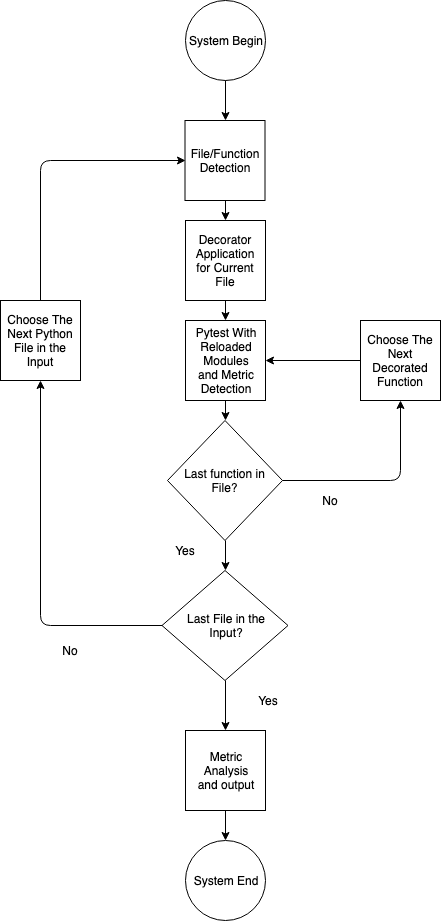
\includegraphics[scale = .6]{images/flow.png}
    \caption{System flow of Function-Fiasco}~\label{systemFlow}
  \end{figure}


% TODO functionality has changed so that the test files are no longer being observed.
  \subsection{System Collection}
    % * System Detection
      The system collection is a process that gives Function-Fiasco the knowledge of what files are being used in the system and the number of functions in each. This process is crucial because it is how Function-Fiasco knows when each file has been analyzed and so it can create a fully examined list of the functions in the system.

    %   * User provided
          Function-Fiasco begins with the user providing the path to the system that the user would like to analyze for pseudo-tested methods. This information is crucial as it provides the location of the root directory of the system and the location of the source code or files. This is accomplished by providing Function-Fiasco a command line argument when starting the system. An example would be \texttt{python3 functionfiasco.py ../fake/ src}.
    %   * Recursive File Exploration
          Once the file path is provided, the next step for Function-Fiasco is file exploration. Since software systems are very complex and could vary in their configuration, Function-Fiasco recursively searches through all paths of the system to find any Python files. The reason that it is looking for this type of file is so that it finds all source code files. It is important to note that test files are ignored from this search. This whole phase can be represented in Figure \ref{systemFlow} as the system begin bubble and the File/Function Detection block. This is because after a new file has been detected, the function detection begins. The function detection process uses AST to search for an AST object called a FunctionDef. This object provides the ability to use the name of the function as it helps to provide the list of associated tests that are pseudo-testing the function. The function detection then provides the number of functions found in each file to give Function-Fiasco the capability of calculating the function coverage for the system. After the functions have been determined in each file, the next step is to begin the analysis for the file that is under scrutiny. This begins with the function and method decoration for that file.

  \subsection{Method Decoration}
  % * File Decoration
    The file decoration phase is one of the most imporant for the execution of Function-Fiasco. This is because Function-Fiasco is using the process for mutation testing and therefore needed a way to analyze a system without altering the source code in a major way. The decoration use in Python was chosen as it is not as intrusive as completely changing the function to eliminate the functionality from it. In fact it provides the ability to maintain the type output that the function would normally have. This type of analysis would allow the testing for other types of ``pseudo-testedness,'' other than the arbitrary check of if the test passes with completely swallowed functionality.

  %   * Per file basis
        The decorator is applied on per file basis. This is in part because of the file exploration. Since Function-Fiasco is using recursive file search to locate all source files, it is helpful to run the analysis on a per file basis to eliminate the number of iterations for the system. It would be unnecessary for Function-Fiasco to find all of the files, then iterate again to add the decorator. On a large system, this process of the double iteration can very quickly become computationally expensive. Another line that is added to each file that allows the decorator to work properly. The line is simply ``\texttt{\textbackslash n \textbackslash n from decorators import skipper \textbackslash n}.'' Without it though, Function-Fiasco would be unable to use the decorator and the system would crash because the applied decorator, \texttt{@skipper}, would be unrecognized.

  %   * All methods receive the decorator
        All functions in the file are decorated at the same time. Function-Fiasco performs one iteration of the file and applies the \texttt{@skipper} decorator call right above every function that is found. This syntax, which can be found in Listing \ref{decoratorExample}, matches the correct usage allowed by Python. Function-Fiasco also has to match the correct spacing of the function that it is being applied to. This is because of the decorators indentation level, the system will crash because it is incorrect usage of the decorator. The reason that they are applied in such a manner is the same as why this is accomplished on the per file basis. The process of adding the decorator, cleaning the file to remove the decorator, and adding it again to the next function would be unnecessarily expensive for the system. Instead Function-Fiasco puts all of the decorators on at the same time and relies on the decorator itself to know if it should apply the manipulation to the file or not.

  %   * Decorator knows what method it should be analyzing
        The decorator is able to accomplish this because functionality has been implemented so that Function-Fiasco knows if the function that is trying to be executed is the file that is currently under scrutiny. Since all tests that are associated with a certain function are executed during the analysis phase it is imporant that any function that is also associated maintains its functionality. So even if 10 methods were executed during the analysis phase, 9 of them would maintain their functionality and the one that does not is masked by the decorator. This is accomplished by adding the name of the function that is currently under scrutiny to the decorator class itself. Since every function is calling to this decorator, the name of all of them is being compared. The only way that the functionality masking and type fuzzing occurs is if the name of the function that is under scrutiny matches the name of the function that is currently being logically determined by the decorator.

  \subsection{Execution and Analysis}
  % * Execution
      The execution phase is where different tests in the test suite of the system are being executed in accordance with the method that is currently under scrutiny. The decorator is meant to do much of the work during the execution, so on the side of Function-Fiasco, there is not much that it needs to do. Function-Fiasco simply runs Pytest in coordination with the aforementioned plugins: PytestFinder and PytestReload. Function-Fiasco provides the method name to PytestFinder and the test suite runs so that only the tests that are associated with the method are executed. This was to cut down on the run time that performing this type of operation can induce. The test suite runs as if the test names were provided. The true execution is performed by the decorator. Since the decorator knows what the correct function to manipulate is, it will allow all other functions to operate as normal but the function that is under scrutiny will have its functionality masked and the return will be fuzzed. After Pytest ends its execution, Function-Fiasco changes the decorator so that the name of the function that was just under scrutiny is forgotten. The analysis is then begun.

  %   * Pytest is run in coordination with PytestFinder and PytestReload
  %   * Method name is given to PytestFinder to reduce the number of tests run
  %   * PER METHOD

  % * Analysis
  %   * Pseudo-tested method data collection
        The analysis begins by collecting the Pytest ouptut from the execution. While Pytest is running, the results of Pytest are being written to a report file so that the results can be examined closer. An example of this report file can be found in Listing \ref{resultOutput}. In this example the output includes which methods were used during the test execution. This information allows Function-fiasco to update the number of used functions so that the coverage may be accurately calculated. The next piece of important information is the test status of \texttt{PASSED}. Function-Fiasco looks for this keyword so that it may update the number of pseudo-tested methods. If this keyword appears on one of the tests, the function is considered pseudo-tested because at least one of the tests is pseudo-testing it. The test name would also be updated to a dictionary entry that contains the name of the function and all of the tests that need to be optimized. This analysis is completed for every function and the results of each are collected and compiled to form an overall assessment of the system and its test suite.

        \begin{figure}[t!]
        \begin{lstlisting}[language = Python, numbers = left, frame = single, caption = Execution of pytestFinder., label = resultOutput]
        ======== test session starts ========
        platform darwin -- Python 3.7.0, Pytest-3.8.0, py-1.6.0, pluggy-0.7.1 -- /usr/local/opt/python/bin/python3.7
        cachedir: .Pytest_cache
        rootdir: /Users/nick/Computer_Science/Function-Fiasco/ffiasco-git, inifile:
        collecting ...

        Methods executed during testing
        #######################
        tester
        #######################
        collected 6 items

        ../fake/tests/test_fake.py::test_tester PASSED [100%]

        ======== 1 passed, 5 warnings in 0.03 seconds ========
        \end{lstlisting}
        \end{figure}


  %   * Update to the number of pseudo-tested methods
  %   * Inclusion of poor tests to the method name
  %   * Repeat of the whole process per file

  \subsection{Results}
  % * Table Creation
      The results phase is based around creating a readable table that developers and testers can use to understand where their system is lacking in terms of testing. It is meant to reflect how the system was operating before Function-Fiasco was run, and what the true behavior is after Function-Fiasco makes observations about the behavior of the system and its test cases.

  %   * Coverage creation
        The first step that Function-Fiasco takes to create the table is to calculate the function coverage of the system. This is accomplished by taking the number of methods that were tested during the execution of the test suite and dividing it by the number of methods. The purpose of this is to allow the user to make a comparison to what amount of the system is believed to be adequately tested. The calcluation is represented as follows:

        \begin{quote}
        \textbf{\textit{Defintion:}} A method \textit{m} $\in$ a program \textit{P} is said to be covered if there exists at least
        one test case \textit{t} $\in$ in \textit{TS}, the test suite of program \textit{P} that triggers the execution of at least one path of the
        body of \textit{m}. \textit{TS} is the test suite of \textit{P}~\cite{vera2017comprehensive}.

        Where (\textbf{\textit{TM}}) is the number of tested methods in \textit{P},

        \begin{equation}
        Coverage = \frac{TM}{NUMM}
        \end{equation}
        \end{quote}

  %   * Collection of the overall number of methods in the system
        The number of overall methods in the system is used as an indicator for the user. It is meant to assist in the explanation of the other metrics, as the user will understand how these numbers are being calculated. The number of methods is collected during the execution of system and is provided to the results phase.

        \begin{quote}
        \textbf{\textit{Defintion:}} The number of methods (\textbf{\textit{NUMM}}) to be produced is representative of the total number of methods in program \textit{P}.
        \end{quote}

  %   * Collection of the number of tested methods in the system
        The number of tested methods in the system is used to explain the coverage of the system. This number is collected during the results of the Pytest run. PytestFinder returns all methods that are used in the test execution, Function-Fiasco collects the names and uses a set for storage to ensure that no functions are double counted.

        \begin{quote}
        \textbf{\textit{Defintion:}} The number of tested methods (\textbf{\textit{NUMTM}}) to be produced is representative of the total number of methods in program \textit{P}.
        \end{quote}

  %   * Collection of the overall number of pseudo-tested methods
        The next step that Function-Fiasco takes is the collection of the overall number of pseudo-tested methods. This number is taken from the dictionary that contains all of the methods and their associated tests that need optimization. This list is comprised during the analysis phase, and it contains the complete list of all of the methods. This is because the results phase occurs after execution and analysis phase, so the list is complete. The length of the list, specifically the amount of keys which comprise the method and tests relationship, is the total number of pseudo-tested methods. Methods that are considered to be not pseudo-tested are not added to this list.

  %   * Create the number of the "truly" tested methods
        After the number of pseudo-tested methods has been collected, the calculation for the number of ``truly'' tested methods can be calculated. This metric is representative of the number of methods in the system that are not being pseudo-tested, but are still being adequately tested by the system. The calculation is as follows:

        \begin{quote}
        \textbf{\textit{Defintion:}} The number of truly-tested methods (\textbf{\textit{NUMTTM}}) to be produced is representative of the total number of adequately tested methods in program \textit{P}.

        \begin{equation}
        NUMTTM = NUMTM - NUMPTM
        \end{equation}
        \end{quote}

  %   * Actual Coverage Creation
        The updated coverage is the overall result of the execution of Function-Fiasco. It is representative of the function coverage with all that are pseudo-tested removed. The updated coverage shows the fault detection effectiveness of the test suite. The calculation is as follows:
        \begin{quote}
        \begin{equation}
        UC = \frac{NUMTTM}{NUMM}
        \end{equation}
        \end{quote}

  %   * Table is created and shown
        Once all metrics have been created, they are compiled into a table, that is shown to the user. The table when compiled can explain the shortcomings in the test suite that is under scrutiny. It provides all pertinent information that can be used to fully examine the test suite. An example of the table is shown in Listing \ref{tableOutput}. Statement coverage for the system has been included in the table. It is important for the user to be able to compare the metric that they have been using previously with the updated metric.

        \begin{figure}[t!]
        \begin{lstlisting}[language = Python, frame = single, basicstyle=\tiny]
   +-----------+----------+---------+---------+----------+---------------+---------+----------+
   | Statement |          |         | Number  |          |    Number     | Number  |          |
   | Coverage  | Initial  | Number  |   of    | Fiascoed |      of       |   of    | Updated  |
   |           | Function |   of    | Tested  |  Methods | Pseudo-tested |  Truly  | Coverage |
   |           | coverage | Methods | Methods |          |    Methods    | Tested  |          |
   |           |          |         |         |          |               | Methods |          |
   +-----------+----------+---------+---------+----------+---------------+---------+----------+
   |    67%    |   0.44   |   730   |   319   |    16    |       9       |   310   |   0.42   |
   +-----------+----------+---------+---------+----------+---------------+---------+----------+
        \end{lstlisting}
        \caption{Example of the table output.}~\label{tableOutput}
        \end{figure}

  %   * Option for the tests that need optimization
        The final part of the overall execution is an option to see the tests that need optimization. This is an option mainly because of the potential length for this section. Computer science systems are very complex and may contain a numerous number of functions and tests. Based on the size and complexity, this list could very easily become long and difficult to read.




%ch:implem
 % Chapter organization is topic-dependent
 %
% $Id: ch03_thework.tex
%
%   *******************************************************************
%   * SEE THE MAIN FILE "AllegThesis.tex" FOR MORE INFORMATION.       *
%   *******************************************************************
%
\chapter{Method of Approach} \label{ch:method}
This chapter is meant to explain the experimentation and testing process. It will discuss many of the decisions for what would be tested and how. It will also explain the qualifications that were necessary for a system to be experimented on.

\section{Test Environment}
% Algorithm \ref{widgmin} (from \cite{Fiori:2013}) shows a high-level description of an
% algorithm. There are many options for the display of
% pseudocode; this uses the {\tt algorithm2e} package \cite{Fiori:2013},
% but there are a number of others available at the Comprehensive \TeX\ Archive
% Network (\url{ctan.org}). Using any of these
% other packages might require the additon of one or more
% ``\verb$\usepackage{...}$'' commands in the main {\tt AllegThesis.tex} file.
% comment for submission
%   *******************************************************************
%   * SEE CHAPTER ch_01overview.tex FOR INFORMATION ON CONTROLLING    *
%   * PLACEMENT OF FIGURES.                                           *
%   *                                                                 *
%   * THERE ARE MANY DIFFERENT ALGORITHM ENVIRONMENTS. HERE, WE USE   *
%   * THE "algorithm2e" PACKAGE, BUT YOU SHOULD LOOK TO SEE IF        *
%   * OTHER PACKAGES BETTER MEET YOUR NEEDS. REGARDLESS OF WHICH      *
%   * PACKAGE YOU USE, EXPECT TO SPEND TIME READING THE USER MANUAL   *
%   * AS THERE ARE USUALLY A LARGE NUMBER OF PARAMETERS THAT CAN      *
%   * SIGNIFICANTLY AFFECT THE FINAL APPEARANCE OF THE ALGORITHM.     *
%   *******************************************************************
A very pivotal part of the system's creation was the testing phase. This phase was meant to determine if the functionality of Function-Fiasco is working properly. This entailed ensuring that Function-Fiasco was operating correctly on many of the different configurations that could be found in software systems, as there are many ways of solving a problem. Since Function-Fiasco is very early on in the developement process, it only works on the primitive data types that exist in Python. These types include \texttt{ints}, \texttt{booleans}, \texttt{floats}, and \texttt{Strings}. Another type of configuration that Function-Fiasco could experience is the use of object-oriented design. An issue arose during the implementation process that involved these methods being looked over when determining which methods could be ``fiascoed.'' This issue pertained to AST not proceeding far enough into the node tree to find that these methods also existed in the system. The final scenario that Function-Fiasco is able to handle is that of a function that is decorated. Applying the decorator to the function involved checking if the function under scrutiny has been decorated, then changing the order of decoration so that the Function-Fiasco generated decorator is closest to the level of the function. Once all of the scenarios had been dealt with, there needed to be a way to determine if the functionality of the system is working properly. There were many different ways that Function-Fiasco was tested which include: a file created that housed the many different scenarios, running the system on the well documented and covered system GatorGrader~\cite{Gat}, and tests written to test the different aspects of Function-Fiasco. These three tests were useful in very different ways. The created file provides the ability to ensure that Function-Fiasco has the ability to handle certain scenarios that it may experience. Running Function-Fiasco on GatorGrader provided the knowledge that Function-Fiasco can operate on large scale systems with a degree of accuracy. Lastly, the different written tests ensure that certain parts of the system are operating the way that they should be by themselves. This is important because it shows that one aspect could be affecting the overall run of Function-Fiasco. This allowed the development process to be handled separately and with greater granularity.

% * Fake test folder
\subsection{Fake Test Folder}
During the development process, a folder was created so that Function-Fiasco could be executed to determine if a recent implementation was working properly on a system that is configured, rather than a file that contains no tests. Configuration is one of the greatest limiting factors when it comes to the execution of Function-Fiasco. It was important to ensure that Function-Fiasco was able to run on at least one configuration. This configuration was one that has the tests in a different directory than the source files. Another portion of the configuration involved the use of \texttt{\_\_init\_\_.py} files, or commonly referred to as dunder files. A dunder file is a file that Python is using in a special way. Pytest is using this file as a manner of marking. This file is meant to point Pytest to return one directory to search for a \texttt{Pytest.ini} file~\cite{okken_2018}. Function-Fiasco is leveraging the dunder files in a very interesting way though. Since it requires that all of the previously loaded modules need to be reloaded, the dunder files indicate where there have been changes made so that the Pytest suite is able to locate the changes. The configuration for the fake test folder can be found in Figure \ref{fakeConf}. This configuration is mostly the standard for systems that are being tested under the Pytest framework. Source files and test files do not need to be in separate folders, but it may make it easier to track the different sets of files as it makes the system more modular. Another reason that the fake test folder was so useful in the creation of the system is that of the representation of the different types of functions that it contains. As mentioned previously, Function-Fiasco is still currently limited to the kinds of functions that it can handle. So it was easy to place them in a file to ensure a multitude of things, such as whether or not the decorator was being applied correctly or if the output after ``fiascoing'' enabled it to determine if the function was being pseudo-tested.


\begin{figure}[t!]
\begin{lstlisting}[language = Python, frame = single]
Fake/
|__ README.md
|__ runfake.py
|__ src/
   |__ __init__.py
   |__ fake.py
|__ tests/
   |__ __init__.py
   |__ test_fake.py
   |__ conftest.py
\end{lstlisting}
\caption{File configuration of the fake system.}~\label{fakeConf}
\end{figure}

The functions found in Listing \ref{fakepy} are meant to test certain things. The first function that is found is not really a function at all. It is a decorator that is meant to be used on the other functions. This function should not be considered in the pseudo-tested method detection and is ignored because the return type is not a callable, so the function is not called. The next function is meant to represent a function that has a return type of an int. Function-Fiasco should detect it and should fuzz the output so that it is still an integer type but is not equal to 6. \texttt{search} is a more unique function in Listing \ref{fakepy}. It is a function that is already decorated, when it is ``fiascoed,'' the decorator that is currently there, \texttt{decorate}, will be placed in the outermost decoration level. This decoration is represented in Listing \ref{multipleDecoration}. \texttt{Addition} will act in the same manner as \texttt{length}, but will fuzz the output of a \texttt{float} instead of an \texttt{int}. The output of the function \texttt{calculate} is unique. The decorator will be applied correctly to the function and it will go through the fuzzing process. The difference is it is a \texttt{boolean} return type. Since there are only two values for a \texttt{boolean}, \texttt{True} or \texttt{False}, the fuzzed return is just the arbitrary integer 10. The next two functions are examples of return types that will not be ``fiascoed.'' One is an object return type, \texttt{tester}, and the other, \texttt{checkOutput}, does not return anything. Both of these types of functions will result in the return type being not recognized and ignored from analysis.


\begin{figure}[t!]
\begin{lstlisting}[language = Python, frame = single, caption = Example of multiple decoration., label = multipleDecoration]
@decorate
@skipper
def search():
    return "asdfjkl;"
\end{lstlisting}
\end{figure}



% ###############################################################################################################
%                                     End of Fake
% ###############################################################################################################

\subsection{GatorGrader}
Another way that Function-Fiasco is being tested is through the execution on another system GatorGrader~\cite{Gat}. GatorGrader is an automated assessment tool that checks the work of programmers and writers. % TODO cite GatorGrader
The main reason that it was chosen was because it fit the same configuration requirements, but at a larger scale. It would allow Function-Fiasco to be tested for its ability to detect the presence of pseudo-tested methods. The process of using GatorGrader began with analyzing the functions and tests present in the system and determinining which functions have the ability of being ``fiascoed''. Out of 91 methods in the source code for GatorGrader, 53 had this ability. The next step in ensuring that Function-Fiasco was operating correctly was ensuring that the decorator was being applied to each of the functions and that each of them was receiving a different output than expected. To accomplish this task, every test had a \texttt{assert False} appended to the end with a print of the output of the function. Then Function-Fiasco was stopped after each file had finished its execution so that a report file that contained the values of the failing tests as well as checking that each function had a decorator applied correctly to it. The final step was running Function-Fiasco on GatorGrader to ensure that the number of pseudo-tested methods was correct. The number of pseudo-tested methods that were found in GatorGrader was 30. An option to produce which functions were being pseudo-tested provided the ability to check each test to determine if the system was correct in determining if the function was being pseudo-tested. This led to many tests being analyzed to find that many of them are swallowing the output of functions just to determine that something was returned. These tests do not check if the output was correct. An example of one of these tests can be found in Listing \ref{swallowedTest}. In this test the function \texttt{get\_details} is being pseudo-tested. Since the assertion is only checking that the output exists, the functionality of the function is not being truly tested. While this function is being pseudo-tested, the purpose of the test is meeting the needs of the developer. After speaking with them they explained that this type of test is to ensure that the system is not crashing. They also explained details of the report in this instance are not relavent to the intention of the test.

\begin{figure}[H]
\begin{lstlisting}[language = Python, numbers = left,frame = single, caption = Test taken from GatorGrader., label = swallowedTest]
def test_commit_checks(reset_results_dictionary):
    """Checks to that invocation of commit check works correctly"""
    invoke.invoke_commits_check(".", sys.maxsize)
    details = report.get_details()
    assert details is not None
\end{lstlisting}
\end{figure}

The final output of the system resulted in a table that appeared as Figure \ref{gatorOutput}. This output is representative of the true behavior that exists in GatorGrader. There are 91 methods that exist in the source code for the system. While the system does have 100\% coverage, there are 78 methods that are being tested by being called explicitly. All methods are being called, but some are being called in a different way, such as being called through a subprocess that executes arguments on the command line. The methods that are being called in subprocesses are being ignored as tested because they are not called explicitly. The number of ``fiascoed'' methods is representative of the number of functions in the system that return a primitive operator and are configured in the way that was previously discussed. An example would be a function that returns an \texttt{int} and is not a generator function. The number of pseudo-tested methods in the case of GatorGrader is 30. Once again, this was at the choice of the developer, but there could be more methods being pseudo-tested because of the parent structure of the system. The parent structure is the idea that functions can call one another. So a function could be directly called by a function that falls under the umbrella of the chosen pseudo-tested methods that are being pseudo-tested because of the structure. The number of truly tested methods that existed was 49, this number was calculated by subtracting the number of pseudo-tested methods from the number of tested methods. Lastly the function coverage was updated to be 53\%.

\begin{figure}[H]
\begin{lstlisting}[language = Python, frame = none,  basicstyle=\tiny]
  +-----------+----------+---------+---------+----------+---------------+---------+----------+
  | Statement |          |         | Number  |          |    Number     | Number  |          |
  | Coverage  | Initial  | Number  |   of    | Fiascoed |      of       |   of    | Updated  |
  |           | Function |   of    | Tested  |  Methods | Pseudo-tested |  Truly  | Coverage |
  |           | coverage | Methods | Methods |          |    Methods    | Tested  |          |
  |           |          |         |         |          |               | Methods |          |
  +-----------+----------+---------+---------+----------+---------------+---------+----------+
  |    99%    |   0.86   |   92    |   79    |    54    |      30       |   49    |   0.53   |
  +-----------+----------+---------+---------+----------+---------------+---------+----------+
\end{lstlisting}
\caption{GatorGrader output.}~\label{gatorOutput}
\end{figure}

GatorGrader's output was used as a control during the development process, partly because the initial errors that Function-Fiasco experienced when testing with GatorGrader would usually fix issues that were found when executing Function-Fiasco on other systems. An example of this is analysis would be ensuring that the import statements that had previously existed in the source files were maintained after Function-Fiasco made alterations.

% ###############################################################################################################
%                                     End of GatorGrader
% ###############################################################################################################

\subsection{Internal Tests}

Another grouping of tests were formed to analyze the portions of Function-Fiasco in their own separate modules. This portion of the testing phase was meant to check the status of implementation changes. It was able to test many manipulations of implementation from new changes to see if they are working correctly, or to see if changes to old functions forced the functionality of other modules to stop working. The creation of pytestFinder was pivotal in this type of testing, as it allows users to perform an impact analysis on changes in a method to determine if they change the functionality of the system. The tests focused on the different phases of the system which include the system collection, method decoration, execution and analysis, and the production of the results.

The system collection phase was created to ensure that the source code of the other system was collected properly. This includes the file walk using \texttt{os} and the function detection and collection using \texttt{AST}. The tests that are checking the file collection are ensuring that every file is being found during the walk of the system. The tests that are checking if the function detection and collection is operating properly are checking each file that exists in the fake folder to ensure that each function is found and that the \texttt{AST} nodes are collecting them and returning the proper amount.

The method decoration is tested in a very different way from the other phases. The other phases rely on running a function and observing the output from the function directly. Testing the method decoration involves running the function that applies the decorator to the file, then comparing it to a file that is the expected output. If each line matches correctly, then the application was successful and the test passes. If any line is off, the test fails. The other methods that support the decorator application, such as one that checks if the line in the file is the correct location to apply a decorator, are tested in similar ways to the other phases.

The execution and analsyis tests involve the functions that are executing the test suites of other systems and the supporting functions that perform the analysis to determine if a function is being pseudo-tested. To perform these tests, the test suite of the other system is run and checked to ensure that it exited properly.

Lastly the functions that are forming the table that is shown to users are tested by checking the values that they produce with different inputs. These tests ensure that the table is being created properly and that the values that are being put into the table are correct and formatted in the proper way.

% ###############################################################################################################
%                                     End of Internal Tests
% ###############################################################################################################

\section{Experiments} \label{sec:Experiments}
An experiment was conducted to determine two things: the ability of Function-Fiasco to detect pseudo-tested methods and the presence of pseudo-tested methods in a variety of sizes and functionality.

% * Projects and their qualifications to be included
\subsection{Projects and Their Qualifications}

When searching for projects to execute Function-Fiasco on, there were certain qualifications that had to be met to be considered a viable candidate for experimentation. The first qualification is that of ease of access. Each candidate needed to be available in an open source fashion from either GitHub or BitBucket. The main reason that this limiting measure was placed was to provide access to the source code in a free and easy way and it allows for the reproduction of the experiment in the future. Reproduction is key because as Function-Fiasco is implemented further, the same systems could be evaluated again to see if there is a noticable difference in the number of pseudo-tested methods.

The next qualification that needed to be met by the candidates was the language that they are implemented and tested in. Since software systems are very complex and may require a combination of languages to complete a task, it was not necessary that Python be the sole language that is used in the system's implementation. To be able to be tested though, each system must be programmed for the majority in Python and it must be tested in a Python based framework. Another aspect of the decision process was trying to make a determination if the size of a system tends to have an impact on the ratio of pseudo-tested methods to number of methods. So the number of methods was taken into consideration when a seemingly viable candidate was found.

The final consideration that needed to be met was the configuration of the system. All systems that are deemed viable must adhere to the file configuration of Figure \ref{fakeConf}. This means that the system must configured in a modular manner. This modular manner also means that there is a dedicated test folder that holds all of the tests separate from the source code of a system. This allows Function-Fiasco to count the number of methods and apply the decorators without also having to check that the function is not a test. The system also needs to be configured to be tested with Pytest. Since Pytest is a very flexible and versatile framework, it has the capability to execute legacy tests that were written in unittest as well~\cite{okken_2018}. This widened the range of possibilites for candidates. Many systems were either tested with just Pytest, or a mixture of both unittest and Pytest. Luckily this ability to execute legacy tests allows Pytest to be executed on systems that are solely tested with unittest.

The final list of used systems can be found in Table \ref{sysList}. Ten systems were chosen as they all met the criteria for testing. It is important to note that the system Hashids-Python needed to have the configuration settings tweeked. Every other system has its source code placed into another directory, Hashids-Python has a single file that contains the source code for the system. Therefore, there does not need to be a dunder file placed in the root directory.

% latex table generated in R 3.4.4 by xtable 1.8-3 package
% Sat Mar 30 16:19:07 2019
\begin{table}[H]
\centering
\begin{tabular}{rlrrr}
  \hline
 & System\_Name & Num\_Methods & Fiascoed & Num\_Tests \\
  \hline
1 & Hashids-Python &  16 &  10 &  59 \\
  2 & Bleach & 368 &   8 & 312 \\
  3 & Pycco &  22 &   6 &  17 \\
  4 & Howdoi &  20 &   2 &  18 \\
  5 & Flashtext &  42 &   7 &  23 \\
  6 & Honcho &  58 &   7 & 124 \\
  7 & Maya &  88 &  13 & 277 \\
  8 & Gator &  91 &  53 & 505 \\
  9 & Hatch & 134 &  14 & 339 \\
  10 & Nikola & 732 &  16 & 205 \\
   \hline
\end{tabular}
\caption{List of systems used for testing.}~\label{sysList}
\end{table}


% ###############################################################################################################
%                                     End of Projects
% ###############################################################################################################

% * Coverage to the new coverage
\subsection{Results of Experimentation}

% * Discovery in almost every system
The execution of Function-Fiasco resulted in the discovery of pseudo-tested methods in almost every system. As previously stated, there were ten executed, all with at least two functions that could be ``fiascoed''. This minimum was placed based on the size of the system. The limit was placed so that there could be a ratio present of how many of the ``fiascoed'' functions were being pseudo-tested. This was so that there could be a basis for how much of the system is truly being affected by the discovery of pseudo-tested methods. Almost every system that was tested was found to have the presence of pseudo-tested methods. The only one that did not have any was the system Howdoi~\cite{Howd}. This can be explained by the low ratio of functions that were ``fiascoed''.

%   * All but one had pseudo-tested methods
%   * Show and explain table that has only the number of ``fiascoed'' and found

The table that contains the information for how many functions were pseudo-tested compared to the number that were ``fiascoed'' can be found in Table \ref{pseudoFound}. Each of them tended to trend upwards with the amount of functions that were ``fiascoed.'' This can be explained by the possiblity of them being found based on the number of functions that were ``fiascoed.'' The systems that had a larger amount of functions to have tested would of course have the higher chance of them being found, purely based on the number being observed. The system with the most pseudo-tested methods found was GatorGrader, but this could be explained by the tests that were meant to check if the system crashed or not. GatorGrader also has a very modular setup, meaning that most methods could be called by any other method to limit the possibility for redundancy. This capability is why so many functions were ``fiascoed''.

% latex table generated in R 3.5.3 by xtable 1.8-3 package
% Tue Apr  2 04:10:03 2019
\begin{table}[H]
\centering
\begin{tabular}{rlrr}
  \hline
 & sys\_name & fiascoed & pseudo \\
  \hline
1 & Hashids-Python &  10 &   8 \\
  2 & Bleach &   8 &   2 \\
  3 & Pycco &   6 &   5 \\
  4 & Howdoi &   2 &   0 \\
  5 & Flashtext &   7 &   4 \\
  6 & Honcho &   7 &   5 \\
  7 & Maya &  13 &   3 \\
  8 & Gator &  54 &  30 \\
  9 & Hatch &  14 &   6 \\
  10 & Nikola &  16 &   9 \\
   \hline
\end{tabular}
\caption{Number of pseudo-tested methods found in each system.}~\label{pseudoFound}
\end{table}



% * Coverage to the new coverage
 % * Discrepancy in the initial function coverage
Many of the systems were not significantly affected by the number of pseudo-tested methods when referencing their function coverage. It is important to note that the function coverage is not consistent with the statement coverage for many of the systems. This can be explained by the number of tests that are not calling functions in a standard way or the number of tests that were not recognized by Pytest because of the configuration. It must also be mentioned that there are cases where the function coverage is higher than the statement coverage of the system. This can be explained by the idea of what function coverage is. Function coverage is how many of the functions are being executed by the test suite. There may be an instance where there is a function that contains many statements that is not being tested, and a function with few statements that is being executed. This scenario would indicate the function coverage being higher than the statement coverage.

The table that holds the information collected from the experiment can be found in Table \ref{fullResult}. This table indicates the change in the function coverage per system. From this table, it can be found that there is an upward trend between systems that boast higher statement coverages and the number of pseudo-tested methods that are found. This is further represented in Figure \ref{stateCovReg}. There was a moderate positive correlation found between the statement coverage boasted from each system and the ratio of pseduo-tested methods to the number of ``fiascoed.'' As the statement coverage of the systems increased, the ratio increased as well. The correlation coefficient between the two variables is 0.45. The systems with the highest statement coverage all were found to have pseudo-tested methods in them, with the highest statement coverages being GatorGrader and Hatch~\cite{Hat}. As shown in Table \ref{sysList}, GatorGrader has 455 tests for just 91 functions and Hatch has 339 tests for 134 functions. These are the two highest when it comes to the number of pseudo-tested methods and the number of tests may be an indication as to why. It could be that the large amount of tests could be creating situations where functions are being pseudo-tested. They are not the most affected by the number of pseudo-tested methods though. With the exception of GatorGrader, systems with less functions had the greater change.

% latex table generated in R 3.5.3 by xtable 1.8-3 package
% Tue Apr  2 04:16:36 2019
\begin{table}[H]
\centering
\begingroup\tiny
\begin{tabular}{rlrrrrrrrrr}
  \hline
 & System\_name & State\_Cov & Function\_cov & NUMM & NUMTM & Fiascoed & Pseudo & NUMTTM & UC & Change \\
  \hline
1 & Hashids-Python & 0.97 & 0.94 &  16 &  15 &  10 &   8 &   7 & 0.44 & 0.50 \\
  2 & Bleach & 0.48 & 0.41 & 368 & 152 &   8 &   2 & 150 & 0.41 & 0.00 \\
  3 & Pycco & 0.77 & 0.86 &  22 &  19 &   6 &   5 &  14 & 0.64 & 0.22 \\
  4 & Howdoi & 0.78 & 0.95 &  20 &  19 &   2 &   0 &  19 & 0.95 & 0.00 \\
  5 & Flashtext & 0.81 & 0.33 &  42 &  14 &   7 &   4 &  10 & 0.24 & 0.09 \\
  6 & Honcho & 0.85 & 0.69 &  58 &  40 &   7 &   5 &  35 & 0.60 & 0.09 \\
  7 & Maya & 0.90 & 0.50 &  88 &  44 &  13 &   3 &  41 & 0.47 & 0.03 \\
  8 & Gator & 0.99 & 0.86 &  92 &  79 &  54 &  30 &  49 & 0.53 & 0.33 \\
  9 & Hatch & 1.00 & 0.56 & 134 &  75 &  14 &   6 &  69 & 0.51 & 0.05 \\
  10 & Nikola & 0.67 & 0.44 & 732 & 319 &  16 &   9 & 310 & 0.42 & 0.02 \\
   \hline
\end{tabular}
\endgroup
\caption{List of results of experimentation.}~\label{fullResult}
\end{table}


\begin{figure}[H]
  \centering
  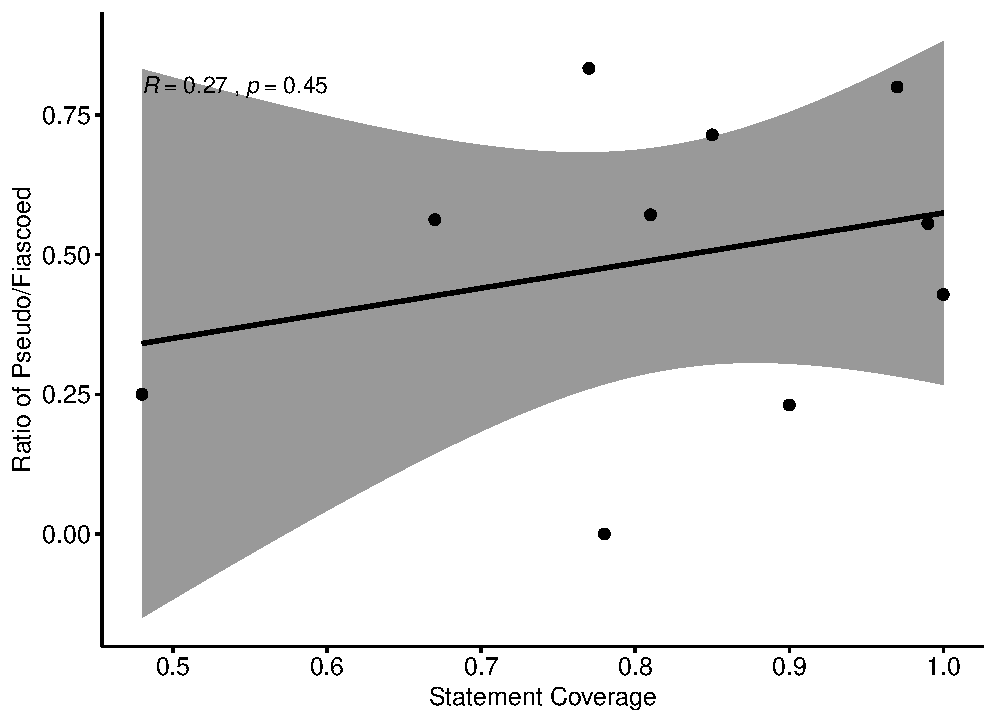
\includegraphics[scale = .5]{images/stateCovPlot}
  \caption{Correlation between the Statement Coverage and a ratio of ``fiascoed'' methods and the number of pseudo-tested methods.}~\label{stateCovReg}
\end{figure}


% * Full result and what it means
The overall result of the experimentation is that pseudo-tested methods are an issue that is affecting systems that are far along in their maturity and systems that are still implementing features. Systems that had lower percentages for their statement coverage were found to have less pseudo-tested methods in their systems. However, this could be explained by the amount of functions that were not being executed as this group could have tested functions in the future that are actually being pseudo-tested. It does follow that the systems that have more tests tend to have more pseudo-tested functions, but this is a product of the sheer number of tests.

The execution of Function-Fiasco resulted in the support for the findings of~\cite{niedermayr2016will}~\cite{vera2017comprehensive}. Both studies concluded with the existance of pseudo-tested methods in Java based systems. The results of this research also concludes that pseudo-tested methods exist in Python based systems. The combination of the findings allows for the inference that pseudo-tested methods can be found in many languages outside of Python and Java. The two languages are completely different when it comes to type safety. Java will force an exception if the type of a variable is overwritten, while Python will allow this computation to occur. There are many languages that are like Java and Python that may experience those same testing vulnerabilities.

It was also discovered that \texttt{Strings} and \texttt{Booleans} are more likely to create a scenario for a pseudo-tested method. For each primitive type of return for functions, the number of the functions present was put into a ratio with the number of functions with that type that were pseudo-tested. Table \ref{retTable} shows a breakdown of the return types that resulted in the most pseudo-tested methods. While some types were used significantly more than others, the ratio of the types explains this reasoning. Both \texttt{Strings} and \texttt{Booleans} are found to produce a pseudo-tested method over half of the time. The number of \texttt{Booleans} that were found to be pseudo-tested may be skewed due to the large number of intentional pseudo-testing that GatorGrader was employing.

% latex table generated in R 3.5.3 by xtable 1.8-3 package
% Tue Apr  2 04:08:23 2019
\begin{table}[H]
\centering
\begin{tabular}{rlrrl}
  \hline
 & Type & Used & Found & ratio \\
  \hline
1 & Strings &  69 &  33 & 47.8\% \\
  2 & Booleans &  49 &  35 & 73.5\% \\
  3 & Ints &  18 &   4 & 22.2\% \\
  4 & Floats &   1 &   0 & 0\% \\
   \hline
\end{tabular}
\caption{Breakdown of the number of pseudo-tested method per type.}~\label{retTable}
\end{table}


%   * In general the systems that have more methods and are further into the maturity of their systems generally contain less pseudo-tested methods
%   * This may be an incorrect statement as the number of functions that can be fiascoified is increased.



% ###############################################################################################################
%                                     End of Experimentation
% ###############################################################################################################
% TODO
% MAYBE ADD THIS SECTION
% * Examples of pseudo-tested methods

% \subsection{Examples of pseudo-Tested Methods}
%
% Since many pseudo-tested methods were found in each system, it is important to mention the different reasons as to why they are being pseudo-tested.

% ###############################################################################################################
%                                     End of Examples
% ###############################################################################################################
%

\section{Threats to Validity}
The threats to the validity of the research are separated into three sections which are based on how the threat would affect the validity of the research. The sections are internal validity, the function coverage, and the confirmability of pseudo-tested methods.

\subsection{Internal Validity}
% TODO determine if the verbage should be researchers or researcher
% * All of the tools that were created to detect the presence of pseudo-tested methods were created by the researcher.
% * Leverages the use of the other made systems, means that if one of them is wrong, the whole result could be

The largest internal threat to validity is the fact that all of the tools that are used in the detection of pseudo-tested methods, with the exception of libraries that are standard to the Python programming language and Pytest, were made by the researcher. This includes the module reloading plugin pytestReload, the impact analysis assistance pytestFinder, and Function-Fiasco which is making the final determination as to what functions are being pseudo-tested. One major effect that this environment can have is the idea that some functions are being left out. Function-Fiasco relies on the passing of test cases to determine if the function is pseudo-tested. There are many tests that pass in the normal setup of the system, but when run from afar with a different configuration the extra step will force them to fail. Which means that the function is not being fully tested for its pseudo-testedness. This could mean that the numbers that were presented in Section \ref{sec:Experiments} could be even higher. Since the research was very intensly tested on the system GatorGrader~\cite{Gat}, which is a system of moderate size with high coverage, it is believed that the number of pseudo-tested methods being present in this system that are untested could be high. This is because Function-Fiasco is very early on in its development maturity. Function-Fiasco is only able to handle a small amount of possibilities when it comes to type returns and object oriented design. This means that many functions in systems, both large and small, are being ignored and not ``fiascoed''. They are still checked to see if they are tested, but they are not analyzed for pseudo-testedness. This means that any of the functions of that are ignored are possibly pseudo-tested.

% ###############################################################################################################
%                                     End of Internal Creation
% ###############################################################################################################

\subsection{Function Coverage}

% * Function coverage does not explain the coverage of a system in a great detail.
%   * Methods that are not tested may not contain a large number of statements, while others do
%   * Blanking

The function coverage that is produced is helpful to understand how many of the system's functions are being tested. This type of insight provides an overhead view of the general behavior of the system. There is an issue with function coverage though, and it is that it is general. One of them most common types of coverage used in industry is statement coverage. Statement coverage is a marker to determine how many of the individual statements are being tested throughout the execution of the system's test suite. This is why the statement coverage of a system could be drastically different from the function coverage. For example, assume there was a function that was not being tested that contains few lines and that there is a function that is being tested that contains a large amount of lines. After the statement and function coverage had been calculated, they would be very different. The function coverage would be affected in a more significant way assuming that there is a small amount of functions in the system. The statement coverage would be affected in a minor way that could be represented with a subtraction of a low number of percentage points. While this would explain the discrepancy in the two types of coverage, it is worth noting because of the adjusted function coverage. To combat this type of threat, the statement coverage is presented to the user as well so that if the function coverage is lower than expected, the user has another metric to base the changes off of.

Another threat to validity involving the function coverage is a term that was created during the implementation phase of the system. This term will be referred to as ``blanking''.  Function-Fiasco relies on the test suite of the system running tests that cause the decorator that is applied to be activated so that the return type of the function under scrutiny is relayed back to Function-Fiasco. If no tests are executed, this return type is ignored and the function is referred to as untested. There is a case where tests are executed for a function, but based on the configuration of the system or tests that were already resulting in a failed case, the test would fail or error before the decorator has the ability to be activated. This would result in the type of the return in the function being relayed to Function-Fiasco as a blank line. Since there were tests executed, the function is still referred to as tested, but it was not ``fiascoed.'' Therefore, this case is referred to as ``blanked''. The blank line is persistant because of the initialization of the variable that stores the return type. It is initialized as an empty string and is unchanged after the execution. This case affects the function coverage because it is still referred to as tested, and forces to the function coverage to remain high. However, the function is not ``fiascoed'' so it is not considered to be checked for its pseudo-testedness. This could result in the function coverage not being accurately corrected after Function-Fiasco finishes its execution.

% ###############################################################################################################
%                                     End of Function Coverage
% ###############################################################################################################

\subsection{Confirmability}

% * Hard to confirm if the output of a large system is correct.
%   * Hand check for pseudo-tested methods to confirm accuracy
%   * Large systems with many require too much time to verify every circumstance
% * Configuration issues may lead to inaccuracy
%   * Based on configuration there may be tests that cannot be run
%   * There is a chance that the fuzzing returned a state that could still be accurate enough to create a passing test case.

Another large threat to the the validity of the research is that the accuracy is very difficult to detect. Since pseudo-tested methods can already be hard to detect by the developer, it is hard to confirm that the system that detects them is working accurately. One major reason is the potential functionality swallowing. It is possible to see that a function is passing a test case when it shouldn't if the test has an assertion that can never fail, but it is difficult to find a function whose functionality is being ignored throughout the systems execution. To accomplish this, a developer needs to follow the execution trail that the function can leave. This means following every function call that the function receives, recognizing what the output should be, and determining if this output truly has an effect on the system as a whole. This can be especially difficult based on the size and the complexity of the system. A function could be used by a numerous amount of other functions. This could make it very difficult to trace the execution trail of a function. It could take too much time and would make using Function-Fiasco redundant. Therefore Function-Fiasco is operating under the assumption that the execution is accurate in detecting pseudo-tested methods with a high degree of certainty. Function-Fiasco has been hand checked on the system GatorGrader~\cite{Gat}, which is a medium-sized system with 100\% coverage and thorough documentation. This means that Function-Fiasco has been checked by hand for a system that contains a plethora of different scenarios to experience.

Another issue that could make it hard to confirm the accuracy of the system is that of configuration issues. It is possible that the configuration of the system that is being tested produces tests that are not able to pass because the configuration from being executed from a directory is not the same as being executed from the root directory of the system. In many cases that are similar to this, the test will error before the function could blank, leaving the possibility of the coverage not being updated to a correct number because of remaining pseudo-tested methods in the system that were not executed. The other threat to the confirmability of Function-Fiasco is the use of fuzzing. Since fuzzing is providing the basis to what is being pseudo-tested or not, there is a chance that the randomized return could create a state that makes the test pass, instead of creating a state where the test should fail but passes anyway. An example of this would be a function that is meant to produce a number within a range, such as an angle for a triangle. In this case any angle that is still valid for a triangle would be accepted and the return produced could satisfy this. To combat this the range that the fuzzing would produce for a number is between 1 and 100, strings are made into an arrangement of random characters, and booleans were returned with an arbitrary number.

% ###############################################################################################################
%                                     End of Confirmability
% ###############################################################################################################

\begin{figure}[t!]
\begin{lstlisting}[language = Python, frame = single, caption = Contents of fake.py, label = fakepy]
def decorate(func):
    def dec(*args, **kwargs):
        return func(*args, **kwargs)
    return dec

def length():
    size()
    return 6

@decorate
def search():
    return "asdfjkl;"

def addition():
    calculate()
    return 5.01019292

def calculate():
    return True

def tester():
    a = classCheck2()
    a.hello2()
    return

def checkOutput():
    return []

class classCheck():
    def hello(self):
        print("hello")

class classCheck2():
    def hello2(self):
        return 10
\end{lstlisting}
\end{figure}
 % Chapter organization is topic-dependent

% YOU MAY HAVE SEVERAL MORE CHAPTERS, DEPENDING ON TOPIC AND ORGANIZATION

%ch:conclusion
%
% $Id: conclusion.tex
%
%   *******************************************************************
%   * SEE THE MAIN FILE "AllegThesis.tex" FOR MORE INFORMATION.       *
%   *******************************************************************
%

\chapter{Discussion and Future Work}\label{ch:conclusion}

\section{Summary of Results}
% A discussion of the significance of the results
% and a review of claims and contributions.

% Significance of results
The results of experimentation support the claims of this research. The research suggested that there are pseudo-tested methods that can be found in systems that are loosely typed. Python is a loosely typed language, and it allows for a variable to be easily overwritten and for a decorator to perform this action.
% Pseudo-tested methods were found in almost every system.
The research has found that pseudo-tested methods were detected in almost every system that was tested. Nine out of ten systems that were tested through the usage of Function-Fiasco had functions that were being pseudo-tested. Overall, out of the 136 functions that were ``fiascoed,'' 72 were found to be pseudo-tested in some fashion. To be considered pseudo-tested the functions needed to be pseudo-tested in at least one test. While this qualification may sound weak, the definition of a pseudo-tested method requires that a test it is executed in will pass regardless of the output of the pseudo-tested method. So while it may be considered strongly tested if the other tests result in a failure, it is still pseudo-tested nonetheless. It is also important to mention the number of pseudo-tested methods found in each system. Function-Fiasco reported low numbers when it ran its execution. Low numbers of pseudo-tested methods in a system is a good thing. This means that the functions that the system is testing can be considered strongly tested. The functions still may be susceptible to other types of errors that result from edge cases, but when considering the expected input into them, the tests execute properly. The fuzzing in Function-Fiasco does perform this edge case exploration, but it is mainly used to determine that any case except for the known input will pass the test.

% Systems that boast high statement coverages tend to have a higher number of pseudo-tested methods
This research also suggested that systems that boast higher statement coverages are found to contain a higher number of pseudo-tested methods. The data produced in this experiment does support this suggestion. It was found that the number of pseudo-tested methods trended upwards as the statement coverage reported by each system increased. An explanation may be that the systems that have higher coverage just introduce more possibilities to pseudo-test functions. This supports the idea that systems that have high coverage are at a greater risk of pseudo-testing their functions. Striving to have a high coverage may lead to writing tests that are not testing something in a meaningful way or accidentally not testing anything at all. It could be argued that the systems with lower statement coverage are writing more meaningful tests that are testing areas that are at great risk in their execution for bugs. Ensuring that every line of code has a test associated with it can also produce a test that is just checking to make sure that something is returned, this can be found in the test suite for GatorGrader. Many of the tests were simply checking that something was returned and that the system did not crash. While these tests do have a purpose, they are considered to be pseudo-tested. This is because they are just checking that something exists, not that what was returned was correct. A test such as this cannot be considered to be fully tested as there is a whole aspect of its functionality that is not being accounted for. Function-Fiasco accounts for the fact that a function is being pseudo-tested by providing an adjusted function coverage that is representative of the actually tested functions of the system.

 % Systems that are using many tests to test one function are producing scenarios where the function is being pseudo-tested
As stated before, the research heavily indicates that the number of tests is the reason for the number of pseudo-tested methods. This is signficant because it means that having meaningful tests is the best practice to ensure that the system is fully testing a function. It is important to say though that statement coverage should also be acknowledged. The purpose of the research was not to explain that statement coverage is a metric that should be ignored. It was meant to leverage the use of statement coverage while still understanding what coverage is. Coverage simply is how much of the system is being executed during the testing phase~\cite{okken_2018}. Coverage is a useful metric, however it does not provide information as to whether or not the test suite has a high fault detection effectiveness. The results indicate this as well. In the systems with the highest statement coverage, almost half of the ``fiascoifiable'' functions in each system were found to be pseudo-tested in some manner. So while it is important to know that all of the system is being executed through the test suite at some point, it does not provide information on the effectiveness of the test suite.

% Why are the results significant
The results of the experiment were significant because they emphasize the danger that pseudo-testing presents. Not every function that was present in every system had the capability to be ``fiascoed.'' If pseudo-tested methods were found in this quantity, the number that may exist in complex systems could be wildly greater than initially expected. Once other types of returns are examined, the number may scale per type. The complexity of the system absolutely plays a role in the number of pseudo-tested methods present. A function may be called indirectly by a wide variety of others, which makes the parent structure that was mentioned before a massive spider web of function calls. This means that a function that is pseudo-tested is affecting much more of the system than thought of before. The number of pseudo-tested methods found in systems with high statement coverage with just primitive types calls for a greater emphasis on the quality of test written. It is very important to understand that the results of this research are an underapproximation. Due to the few cases that Function-Fiasco can handle, there is the possiblity that there are more cases that could lead to further discovery of pseudo-tested methods in a system. The number of pseudo-tested methods that Function-Fiasco will find after further development will not diminish as the further development will only increase the number of functions that can be investigated.

% Major Contributions
The major contributions of this research is as follows:

\begin{enumerate}
  \item A working automatic detection tool for pseudo-tested methods.
  \item A table that contains the results of a system's coverage and fault detection effectiveness.
  \item A revised metric that describes how accurately a system is able to detect errors.
  \item Two Pytest plugins that aid in the testing of software.
\end{enumerate}


\section{Discussion}
% Field Connections
  % * Software Engineering
This research is heavily connected to the field of Software engineering. Software engineering may be defined as the systematic design and development of software products and the management of the software process~\cite{IEEE}. This design is employed using aspects of many other processes that are crucial to the creation of software. The different aspects include design, architecture, implementation and testing. Function-Fiasco connects by examining the result of these processes to ensure that the system that was designed is behaving as the developers have envisioned. It also aims to ensure that the systems that the developers have put in place to check this behavior is written in a way that allows developers to accurately detect faults in their implementation. Overall, Function-Fiasco applies to the field of Software engineering because it is a system that developers can use to ensure that they have implemented their source code so that it acts in the way that was first perceived. It can be used at any point in the implementation if there are test cases that exist already, as this is the workflow that test-driven developement follows.

% * Software Testing
Function-Fiasco is also very heavily connected to the field of Software testing. How development teams test their software can influence the overall product after the development process has completed. It is the process of ensuring that the functionality of the system that has been created is operating in a manner that was intended and expected. This aspect of the development cycle can help to avoid major issues in the execution of the system, such as a crash. It can also ensure that the output of the system is what was expected. If this phase is not accomplished correctly or even at all, the software should be considered unstable to a point where the output in the scenarios that were expected may not be what is provided to the user. Assuming that the developers have written tests for their systems, Function-Fiasco can be used to ensure that the tests have been correctly implemented. Since test suites can be considered an examination of the system, and is often created by the team that developed the software that the test suite is analyzing, it is important to ensure that the tests have been written in a manner that is actually testing the behavior of the system. Function-Fiasco determines if the tests that exist in the test suite are of good quality. It can help determine what is not testing anything so that the tests can be addressed and the function can have proper tests written for it so that the output is being accurately tested.

% * Computer Science
Function-Fiasco is also connected to the greater field of computer science. Software is the way that the user interacts with the hardware in the computer system to perform a meaningnful operation. Function-Fiasco now provides a way to automatically detect faults in a test suite. This means that the developement process has another tool that allows developers to ensure that the software that they are creating is operating properly. This research also shows that the idea of a pseudo-tested method is not localized to the Java language, as this was proven in \cite{niedermayr2016will}. Psuedo-tested methods could potentially be an issue in a wide variety of software that is outside of the umbrella of Python and Java based systems. This greatly affects the field of computer science. This research also calls into question the current metrics that developers can use to ensure that their system is being tested. This extends to languages outside of Java and Python.

% Major Implications
This research could have major implications based on its results and the results of its predecessors. It has been proven that pseudo-tested methods exist in systems that have both high and low percentages of coverage.
  % * Change in the view of tested software
  This means that the definition of tested software stands to change. Currently high coverage can be observed as an indication of testedness. However as proven with this research, high coverage can also create scenarios in which functions of the system are not being adequately tested. Testedness should be reflected by the fault-detection effectiveness of the system. This research also suggests a change in how tested software is viewed. Bugs are common in software, this is because the development process of a system is never finished. After the development cycle has completed, the maintenance of the system begins. In this phase, bugs are made aware to the development team. Once the bugs have been signaled, the developement process cycles and begins again. This process continues because bug fixes involve more implementation that could result in further bugs. There is also the issue of technical debt. Technical debt is defined as code that may currently be working, but in the future, after additional development, may not function as intended~\cite{verdecchia2018architectural}. Pseudo-tested methods may be hiding operations that can be defined as technical debt. Since they are pseudo-tested, even after they are not behaving as they should, they will still result in passing tests. For these reasons, the research conducted with Function-Fiasco has revealed potential flaws in how developers view tested software.

  % * Possible change in the software testing process
  Function-Fiasco also presents the possiblity to change how the process of software testing is operated. Testing in most software engineering models happens late in the developement cycle. Function-Fiasco provides a tool to test not just the system source code during this phase. It allows for the testing of the test suite as well. Analyzing the test suite of systems should also be performed in the development cycle. This is because the tests are how the functionality of the system is determined to be correct. Integrating the process of evaluating the suite into the overall testing phase is imperative. It should not be assumed that functionality is correct until the tests are determined to be written correctly as well. This idea works properly even if the development team is operating under test-driven development. Once the tests are written and functionality begins development, it is easy to test the suite as well. After functionality that fits the test is written, the test could also be analyzed at the same time. This would allow further development knowing that the functionality is implemented properly to a higher standard of certainty. The research performed in the developement of Function-Fiasco and the experiment that followed allows the capability to change the way that the testing process of systems is conducted. It would allow a higher degree of certainty that the system is operating properly.

\section{Future Work}
The implementation on Function-Fiasco and its supporting plugins is not finished and there are many plans for further work on them as well as plans for future testing after these changes are implemented. There is much work that can be done in terms of features and bug fixes. Each addition or fix may lead to further pseudo-tested methods being found in each system.

% Bug Fixes and feature implementation ~ Function Fiasco
Function-Fiasco is the flagship system in the Function-Fiasco organization and it stands to have the most amount of work completed on it. Function-Fiasco has a number of features that need to be added to its functionality so that the system is able to analyze more functions and tests than it currently does.
% Update to the different types that are availble for fiascoifying
The main work that needs to be accomplished is an update to the different function returns that are not being currently analyzed. As stated before, the only functions that can be tested are ones that return a primitive type which include \texttt{integers}, \texttt{floats}, \texttt{booleans}, and \texttt{Strings}. Other types of functions that the system needs to be able to handle are ones that return container objects such as \texttt{lists}, \texttt{sets}, \texttt{tuples}, and \texttt{dictionaries}. The reason that these containers have been chosen is because they can be easily indexed in different ways. The most complex type out of this grouping is the \texttt{dictionary}. The reason being is that each index is a key-value pair, which may be difficult to fuzz depending on what each part of the key-value pair is. After the different container objects are implemented, the next feature that Function-Fiasco needs to be able to handle includes objects that have attributes. This was left out due to time constraints, but it will work in the same fashion as a list. Function-Fiasco will systematically proceed to fuzz each attribute that the object has. This is to ensure that whatever aspect of the function is being tested, the test will have an input of a fuzzed variable.
% Parameterized testing
The next crucial feature that will be implemented into Function-Fiasco will be the ability to discern paramaterized tests. Currently, each test in the paramaterized grouping must pass for the test to be considered pseudo-testing a function. In the future, each test will be looked at as its own entity and the input that the test uses will be used to separate the test grouping.

Function-Fiasco also needs to have an update in the number of tests that it discovers and the number of tested functions that it returns. Currently the number of tested functions of the systems is lower than expected. Systems that have a coverage of almost 100\% are being found to have a function coverage that is not near the 100\% coverage that is expected. This has a direct effect on the metrics that are being produced from Function-Fiasco. The function coverage after Function-Fiasco completes its execution is only going to be diminished due to the presence of pseudo-tested methods. Therefore the initial function coverage and the updated function coverage may be lower than expected. A reason that this may be occuring could be an issue in either pytestFinder or Function-Fiasco. Based on the configuration of some of the systems, running in another directory with a different environment may cause some of the tests to not execute properly. They may be looking for certain conditions that the current evironment does not have, causing the test to error and not release any information on what functions were tested in that execution. This would cause the function coverage to not be as high as it could be because functions were not counted because of the errors. Another issue that may be causing the lower function coverage would be the function discovery in the tests that are produced by pytestFinder. PytestFinder produces only the tests that need to be run because of what functions are being called in them. If pytestFinder does not correctly find all of the function calls in the test, the test will not be run. If this happened throughout the execution for that function, it would not be recognized as tested. Fixing this issue would cause all metrics associated with the number of functions that are tested to increase.

  % Ability to operate on other OS
  A bug that needs to be fixed is what operating systems Function-Fiasco is compatible with. As of now, the only operating system that Function-Fiasco will operate on is MacOS. The plan to fix this bug is to investigate the versions of the dependencies that each system is using. If this is an issue, Function-Fiasco will be shipped with a requirements document that has the updated versions that Function-Fiasco is currently using on MacOS. The other possiblity that may be forcing this issue could be that packages that are downloaded in the system are running at the same time forcing those that Function-Fiasco requires to operate to fail. The fix for this would be to observe what packages are running during the time of Function-Fiasco to determine where the issue is.

  % Documentation
  The documentation for Function-Fiasco needs to be updated as well. Much of the developement for Function-Fiasco was causing functionality to change at a rapid pace. Documenting the changes became an almost sisyphean task. Once the documentation could have been updated and correct, the functionality would change or a dependancy would be added. Therefore the documentation phase of development was difficult to maintain.

% Bug Fixes and feature Implementation ~ pytestFinder and pytestReload
Both pytestFinder and pytestReload need to have documentation updated as both have changed drastically since their conception. However the most significant portion of future work for both of the plugins is a feature that had to be removed from pytestFinder to ensure that the numbers were correct for the experimentation. The beginnings of a system to determine what functions were specifically called during a test were being implemented. This would allow pytestFinder to determine which functions were called based on the logic of the system. As of now, pytestFinder determines which functions and test to run based of AST nodes from the tests and source code. In the future, pytestFinder needs to determine what tests to include in the execution based on what will actually be executed based on the input of each test. This would also aid in the creation of the feature that allows Function-Fiasco to execute paramaterized tests on an individual basis, rather than the whole grouping. This whole grouping forced Function-Fiasco to count more pseudo-tested methods than actually existed.

  % Missed tests and not accurate function coverage
% Additional testing on other open source systems
The final piece of known future work is that of retesting. As more features are added to the functionality of Function-Fiasco, the same systems need to be examined again to determine if the current claims from this research remain consistent as the number of ``fiascoed'' functions increase. As stated previously, the planned future development involves adding cases that Function-Fiasco can handle. This development would expose other parts of the systems to further scrutiny that was not possible prior at the time of writing. This increase in scrutiny will result in the number of ``fiascoed'' methods increasing, and in theory increasing the number of pseudo-tested methods. Further examination of systems with Function-Fiasco could potentially have a greater affect on the coverage that the systems boast. This information would only support the idea that pseudo-tested methods are a prevalent issue that needs to be addressed. It will also provide more insight on which return types are the highest danger of pseudo-testing.

Research should also be performed on the different types of coverage. Even though statement coverage is a widely used metric to determine how much of a system is being tested, it is not the most stringent. There are other types of coverage that are more stringent and encompassing than statement coverage, such as fully defined mutation testing and modified condition coverage. When using other types of coverage that are more stringent, research may show that systems that still have a high coverage may have less pseudo-tested methods present due to more conditions being checked.


\section{Conclusion}
% Overall issue of pseudo-tested methods
The purpose of this research was to prove that pseudo-tested methods exist in systems that are based in Python. The experimentation proved this. Pseudo-tested methods were found in almost every system, regardless of the size or statement coverage. Out of the 10 systems that were examined, 9 were found to include functions that were being pseudo-tested. This finding is very important as it shows that this is an issue that is very prevalent and needs to be addressed. The idea of pseudo-tested methods was not conceived until 2016~\cite{niedermayr2016will}. They are a very new idea in computer science and are not being acknowledged in great detail. This research shows that the way that development teams are testing their software is creating cases that are not fully analyzing the behavior of the system.
 % * Pseudo-tested methods are a prevelant issue
 % * Found in almost every 9/10 systems that were tested

% Updated understanding that coverage could be a misleading metric
This research was also meant to provide insight into an aspect that coverage may not be providing information for. The fault detection effectiveness of a system may not always be indicated by the coverage of a system. A system having 100\% coverage does not mean that the tests that it is employing can be considered good tests. As shown previously, some tests were merely created so that the developer can determine if the system is simply returning something as an output. This can be seen by tests in GatorGrader that are just ensuring that the count of an element is greater than one. A case that this allows the test to pass is a number that can be considered high for the system. Since it is allowing information that is greater than the number one, if the system counts too many items, the number that is being compared may be very high. This will still pass the test case. While the test is accomplishing what the developer intended, it is still not ensuring that the number that it receives is correct. This research also found that the systems with the highest percentage of statement coverage had the highest number of pseudo-tested methods contained in their source code. These aspects suggest that more should be considered when determining if the system is being tested thoroughly. This research does not conclude that coverage is always misleading. It is still important to understand how much of the system is under scrutiny. The point of the research was to provide insight into the fault detection effectiveness of test suites.
 % * Systems with higher statement coverage had more pseudo-tested methods
 % * Some tests were used to ensure that the system did not crash

The findings of Function-Fiasco have also supported many of the conlcusions that were made in past studies. Chapter \ref{ch:relatedwork} presented the related work that has already been completed on this topic. Those studies have proven that pseudo-tested methods exist, specifically in Java based systems. They also provided a rationale that coverage may not always be a misleading metric. The research conducted during the execution of Function-Fiasco prove that pseudo-tested methods exist in Python based systems. A very interesting observation is made in \cite{vera2017comprehensive} is that other languages than Java may contain pseudo-tested methods. They concluded that their research could not be generalized to other languages. Their work was limited to the Java programming language, so they were not able to conclude if the same conditions could be found in other languages. Function-Fiasco has not only supported their research to prove that pseudo-tested methods exist, but it shows that this is an issue that is not only limited to Java. Function-Fiasco also supports the idea coverage as a metric is not an entirely misleading metric. Coverage is useful in understanding how much of the system is being executed during the evaluation of a system, but it does not indicate that the test suite has a high fault detection effectiveness.

% Ability to test for them automatically
Lastly, Function-Fiasco provides developers a way to evaluate their test suites. Prior to Function-Fiasco, the most commonly used metric was that of coverage. The issue with coverage is that it does not provide an indication as to the fault detection effectiveness of the system. Coverage cannot determine the quality of the tests, only how much is being tested in them. Function-Fiasco has the ability to determine the quality of the test, which means is it actually testing what was intended. Based on the size and complexity of systems, it can be very difficult to check each of the systems by hand. Pseudo-tested methods by nature are difficult to find because they are masked by a continuously passing test case, so checking for them by hand may not find all of them. It will also take a long time to check every case, and by the time this has been accomplished, the test suite may have changed forcing the evaluation to begin again. Function-Fiasco provides the ability to detect pseudo-tested methods automatically. It finds pseudo-tested methods using a combination of mutation testing, fuzz testing, and fault injection to determine if a function is being tested properly.
 % * Nearly impossible to test each of the cases of a pseudo-tested method by hand
 % * Function-Fiasco presents the possibility of testing for these functions automatically
 % Conclusion/future work

%   ********************************************************************
%   * IF YOU HAVE ANY APPENDICES (FOR INSTANCE, CODE, DATA, GRAPHS,    *
%   * OR ANYTHING ELSE THAT DOESN'T "FIT" AS REGULAR CHAPTER CONTENT), *
%   * INCLUDE THE FOLLOWING LINE, WHICH INSTRUCTS LATEX TO CHANGE FROM *
%   * NUMBERED "CHAPTER" HEADINGS TO LETTERED "APPENDIX" HEADINGS.     *
%   *                                                                  *
%   * APPENDICES HAVE THE SAME FORMATTING COMMANDS AS CHAPTERS (E.G.,  *
%   * "\chapter{...}", "\section{...}", ETC.)                          *
%   ********************************************************************

\appendix

%
% $Id: appa--code
%
%   *******************************************************************
%   * SEE THE MAIN FILE "AllegThesis.tex" FOR MORE INFORMATION.       *
%   *******************************************************************

% \chapter{Java Code}\label{appa:code}
% All program code should be fully commented. Authorship
% of all parts of the code should be clearly specified.
%
% %   *******************************************************************
% %   * SEE THE MAIN FILE "AllegThesis.tex" FOR THE "\lstset" COMMAND   *
% %   * THAT DEFINES HOW PROGRAM LISTINGS WILL LOOK.                    *
% %   *******************************************************************
%
% % \lstinputlisting{SampleProg.java}
  % Appendices go here

%   ********************************************************************
%   * THE FINAL COMMANDS DEAL WITH BIBLIOGRAPHY/REFERENCES. IF THERE   *
%   * ARE ANY ITEMS IN YOUR BIBTEX FILE THAT YOU DID NOT REFERENCE IN  *
%   * YOUR PAPER, BUT THAT YOU WISH TO INCLUDE IN THE BIBLIOGRAPHY,    *
%   * YOU MAY SPECIFY "\nocite" COMMANDS TO FORCE THEM TO BE INCLUDED. *
%   *                                                                  *
%   * THE COMMAND "\nocite{*}" FORCES EVERY ITEM IN YOUR BIBTEX FILE.  *
%   ********************************************************************

%\nocite{ckm-acmap-99}   % EXAMPLES OF FORCING THINGS TO BE INCLUDED
%\nocite{Dierckx93}      %   "   "   "
%\nocite{obs-stcav-92}   %   "   "   "
%\nocite{bb4471}         %   "   "   "

\nocite{*} % OR DO THIS TO INCLUDE ALL BIBTEX REFERENCES IN THE BIBLIOGRAPHY

%   ********************************************************************
%   * IF YOU HAVE YOUR BIBLIOGRAPHY IN A SEPARATE ".bib" FILE, HERE IS *
%   * WHERE YOU MUST SPECIFY IT. IN THIS EXAMPLE, THE BIBLIOGRAPHY     *
%   * ENTRIES ARE STORED IN A SUBDIRECTORY NAMED "Bibdir" IN A FILE    *
%   * NAMED "myBibtexDB.bib".                                          *
%   ********************************************************************

\begin{spacing}{1}
\bibliographystyle{plain}
\bibliography{Bibdir/myBibtexDB}    % File type ".bib" is assumed
\end{spacing}

\typeout{THEPAGE \thepage}

\end{document}
